\part{Thermodynamics}\label{Thermodynamics}

\section*{Introduction}

This section of the course was lectured by \href{https://users.physics.ox.ac.uk/~pierrehumbert/}{Raymond T. Pierrehumbert} covering basic Atmospheric Thermodynamics. While most concepts here will be applicable to oceanic physics, we will only be explicitly applying the concepts learnt in this section to atmospheric physics.\vspace{5 mm}

\noindent This section consists of three chapters:\vspace{5 mm}

\begin{enumerate}
    \item \hyperref[Basic Thermodynamics]{Basic Thermodynamic Concepts}: 
        
        \begin{quote}
            We recap some basic thermodynamic concepts you should be familiar with, like pressure, \hyperref[Ideal Gas Box]{ideal gases}, and \hyperref[Equipartition]{heat capacity}. We then explain how to extend such concepts to deal with gases consisting of \hyperref[Definition Multiple]{multiple constituents}. Finally, we introduce the important approximation of \hyperref[Hydrostatic Box]{Hydrostatic Balance}.
        \end{quote}

    \item \hyperref[Dry Thermodynamics]{Dry Thermodynamics}: 
    
        \begin{quote}
            We focus primarily on the vertical temperature structure of the atmosphere. We predict and explain some observations by deriving the \hyperref[Dry Adiabat Box]{Dry Adiabat}, which governs the temperature of a convecting parcel of air. Next, we consider convection, and derive a \hyperref[Dry Stability Box]{criterion} of whether an atmosphere will be unstable to convection and define a \hyperref[Convection Box]{few terms} relating to convection.
        \end{quote}
    
    \item \hyperref[Moist Thermodynamics]{Moist Thermodynamics}:
        \begin{quote}
            We extend the previous section to apply to atmospheres which have constituents which condense. We derive the \hyperref[Moist Pseudo Adiabat]{Moist Pseudo-Adiabat}, the moist counterpart to the \hyperref[Dry Adiabat Box]{Dry Adiabat}. We do not discuss moist convection here, and instead discuss this in Part \ref{Clouds}.
        \end{quote}
\end{enumerate}

\chapter{Basic Thermodynamic Concepts}\label{Basic Thermodynamics}

\section{Definitions}

\subsection{Basic Thermodynamic Definitions}

We should review (or learn) the basic state variables of thermodynamics. 

For Atmospheric and Oceanic Physics, we will almost always work with `\textit{Intensive}' variables. These are variables that are independent of the size of a system. For example, `number of particles' is not an intensive variable, because the number of particles changes (it doubles) if you double the size of the system. However, `number of particles \textit{per unit volume}' is an intensive variable, because this remains unchanged when you double the size of a system.

As a brief review, we'll need to know the following \textit{intensive} variables:
\begin{table}[h!]
    \begin{tabular}{|p{1.4cm}|p{2.8cm}|p{4cm}|p{7.4cm}|}
    \hline
        Symbol & Name & Units & Meaning \\
    \hline
    \hline
    $p$ & Pressure & \qty{}{\pascal} (Pascal); \qty{}{\bar} (Bar); \qty{}{\newton\per\square\metre} (Newtons per square metre); & The force exerted by the fluid in \textit{all} directions at some location. \qty{1}{\bar} $\approx$ \qty{e5}{\pascal}. \\
    \hline
    $T$ & Temperature & \qty{}{\kelvin} (Kelvin) & A measure of the heat content of the system. \\
    \hline
    $\rho$ & Density & \qty{}{\kilogram\per\metre\cubed} (Kilograms per metre cubed) & The mass per unit volume.\\
    \hline
    $n_a$ & Number Density & \qty{}{\per\metre\cubed} (Inverse metre cubed) & The number of molecules of some substance $a$ in one metre cubed. \\
    \hline
    $M_a$ & Molar mass & \qty{}{\kilogram\per\mole} (Kilograms per mole) & The mass of $N_A\sim$ \qty{6.02e23}{} molecules (one mole) of $a$.\\
    \hline
    \end{tabular}
    \caption{Basic Intensive Thermodynamic Variables}
\end{table}

Note that many resources present the molar mass $M_a$ in units of \qty{}{\gram\per\mole} (grams per mole). This is in order to produce more pretty numbers: for example, the molar mass of N$_2$ is \qty{28.01e-3}{\kilogram\per\mole} $=$ \qty{28.01}{\gram\per\mole}. However, be wary of units, and always remember to convert everything to SI units when doing calculations. For this you can simply divide the molar mass in units of \qty{}{\gram\per\mole} to units of \qty{}{\kilogram\per\mole} by dividing by $1000$:
\begin{align*}
    \underbrace{M_a}_{M_a\text{ in SI units of \qty{}{\kilogram\per\mole}}} = \underbrace{M_a}_{M_a\text{ in non-SI units of \qty{}{\gram\per\mole}}}\cdot\frac{\qty{1}{\kilogram}}{\qty{1000}{\gram}}
\end{align*}

\subsection{Multiple Constituents}\label{Multiple}

In general, a planet's atmosphere is composed of multiple constituents. Our goal is to expand our vocabulary to describe the abundance of a certain constituent in the atmosphere.

It turns out that we (or the examiner) must make two ultimately arbitrary decisions if we wish to refer to a certain constituent's abundance. First, we can either refer to a constituent's abundance by its \textit{mass}, or by it's \textit{number} (in \textit{moles}). Second, we can either refer to it as a \textit{concentration} or a \textit{ratio}. These choices are ultimately arbitrary because one may freely convert between them with the molar mass using Equation \ref{density to number}.

Suppose our atmosphere is composed of constituents  $\mathbb{S}=\{a,b,c,\ldots\}$. Each species $i\in\mathbb{S}$ has a molar mass of $M_i$ and a number density of $n_i$. Then we can refer to it's abundance as follows. All quantities are dimensionless.

\begin{fact}{Definitions Regarding Constituent Quantities}{Definition Multiple}\label{Definition Multiple}
    We can refer to the amount of a certain constituent $a$ in an atmosphere as follows:\newline\newline
    \begin{tabular}{|p{0.8cm}|p{6.5cm}|p{7.5cm}|}
        \hline
        & Fraction/Concentration & Mixing Ratio \\
        \hline
        Mole & \textit{Mole Fraction} or \textit{Molar Concentration} \begin{align*}
            x_a=\frac{n_a}{\sum\limits_{i\in\mathbb{S}} n_i}
        \end{align*} & \textit{Molar Mixing Ratio} or \textit{Volume Mixing Ratio} \begin{align*}
            \frac{n_a}{\sum\limits_{i\in\mathbb{S},i\neq a} n_i}
        \end{align*}
        \\
        \hline
        Mass & \textit{Mass Fraction} or \textit{Mass Concentration} \begin{align*}
            q_a=\frac{\rho_a}{\sum\limits_{i\in\mathbb{S}} \rho_i}
            =
            \frac{M_an_a}{\sum\limits_{i\in\mathbb{S}} M_in_i}
        \end{align*} & \textit{Mass Mixing Ratio} \begin{align*}
            \frac{\rho_a}{\sum\limits_{i\in\mathbb{S},i\neq a} \rho_i}
            =
            \frac{M_an_a}{\sum\limits_{i\in\mathbb{S},i\neq a} M_in_i}
        \end{align*}\\
        \hline
    \end{tabular}\newline

    where $n_i=$ the number density of $i$; $M_i=$ the molar mass of $i$; and $\rho_i=$ the density of $i$. We let $x_a$ and $q_a$ refer to the mole fraction and mass fraction of $a$, respectively.

    All formulations are equivalent, as one can freely convert between all four expressions using algebra or by using the following formula:
    \begin{align}\label{density to number}
        \rho_A=\frac{n_AM_A}{N_A}
    \end{align}
    where $N_A=\text{Avogadro's Number}\sim$ \qty{6.02e23}{\per\mole} (it's on your formula sheet).\footnote{
        To avoid a small confusion, note how only number density $n_i$ is used in the definition for the \textit{molar} concentrations/mixing ratios. This is because the number of moles per volume of a substance is directly proportional to the number density: $n_i^{mol}=n_iN_A$. As such the $N_A$'s simply cancel top and bottom in the fraction.
    } 
\end{fact}

We also introduce the concept of '\textbf{dilute}': some constituent $a$ is in the \textbf{dilute} limit if and only if:
\begin{align}\label{Dilute}
    \boxed{n_a\ll\sum\limits_{i\in\mathbb{S},i\neq a} n_i\hspace{10mm}\text{and/or}\hspace{10mm}
    \rho_a\ll\sum\limits_{i\in\mathbb{S},i\neq a} \rho_i}
\end{align}

An important upshot of this is that, in the dilute limit, fractions/concentrations and mixing ratios are equivalent. In many problems, this simplifies the algebra massively, but you're not always allowed to assume that constituents are dilute (especially in exams!).

Note however that there is some ambiguity in the 'and/or' in Equation \ref{Dilute}. For example, we might have a situation where $n_a\ll\sum n_i$ but \textbf{not} $\rho_a\ll\sum \rho_i$ (or vice versa). This occurs only if the molar masses $M_a$ and $M_i$ are not all of similar size (convince yourself that this is the case using Eqn. \ref{density to number}). This is almost never the case in scenarios we consider, so you can just treat the `and/or' as just an `and' in Equation \ref{Dilute}.

Sometimes, we'll see people refer to dilute constituents in terms of \textit{ppm} (parts per million) or \textit{ppmv} (parts per million volume). \textit{ppm} is defined as the \textit{Mass Fraction} or \textit{Mass Concentration} multiplied by $10^{6}$ ($q_a\times10^6$) while \textit{ppmv} is defined the \textit{Mole Fraction} or \textit{Molar Concentration} multiplied by $10^{6}$ ($x_a\times10^6$).

\subsubsection{Atmospheric Composition: Planetary Examples}

In \textit{Mole Fraction} $x_a$:
\begin{multicols}{2}
\begin{itemize}
    \item Earth's Atmosphere: 
    \begin{itemize}
        \item Nitrogen N$_2$: 0.78
        \item Oxygen O$_2$: 0.21
        \item Argon Ar: 0.0093
        \item Carbon Dioxide CO$_2$: 0.000430 (430 \textit{ppmv})\footnote{At time of writing!}
        \item Water Vapour H$_2$O: A few percent.\footnote{This strongly depends on time and location due to dynamics discussed in \hyperref[Moist Thermodynamics]{Moist Thermodynamics}.}
    \end{itemize}
    \item  Venus' Atmosphere:
    \begin{itemize}
        \item Carbon Dioxide CO$_2$: 0.965
        \item Nitrogen N$_2$: 0.035
        \item Sulfur Dioxide SO$_2$: 150 \textit{ppmv}
    \end{itemize}
    \item  Jupiter's (Outer) Atmosphere:
    \begin{itemize}
        \item Hydrogen H$_2$: 0.86
        \item Helium He$_2$: 0.136
    \end{itemize}
\end{itemize}
\end{multicols}

\section{Ideal Gases}

\subsection{Single Constituent Atmosphere}

An \textbf{Ideal Gas} is a theoretical (imaginary) gas consisting of molecules which interact only via perfectly elastic collisions. No real gas is ideal, but many gases, including 99\% of Earth's atmosphere (Nitrogen, Oxygen, and Argon), behave approximately like ideal gases under atmospheric conditions like ours. We start from the version of the ideal gas law that you've probably seen before, and assume that the gas is made up of a single constituent $a$ for simplicity:
\begin{align}\label{Ideal Gas Primitive}
    \boxed{pV=N_ak_BT}
\end{align}
where $p=$ pressure, $V=$ volume, $N_a=$ number of molecules of $a$, $k_B=$ Boltzmann's constant, and $T=$ temperature. We can divide by the volume, then multiply and divide by $\frac{M_a}{N_A}$ to get: 
\begin{align*}
    p&=n_ak_BT & \text{; }&\text{Divide \ref{Ideal Gas Primitive} by }V\\
    &=\left(\frac{n_aM_a}{N_A}\right)\left(\frac{k_BN_A}{M_a}\right)T&\text{; }&\text{Multiply and divide by }\frac{M_a}{N_A}\\
    &=\rho_a\left(\frac{k_BN_A}{M_a}\right)T & \text{; }& \text{Use \ref{density to number} to substitute for }\rho_a\\
    &=\rho_a\left(\frac{R^*}{M_a}\right)T
    &\text{; }&R^*\equiv k_BN_A=\text{gas constant}\\
    &=\rho_aR_aT
    &\text{; }&R_a\equiv\frac{R^*}{M_a}=\text{specific gas constant}
\end{align*}

The \textbf{Gas Constant} $R^*$ is defined as: $R^*\equiv k_BN_A\approx$ \qty{8.314}{\joule\per\mole\per\kelvin}. We further define the \textbf{Specific Gas Constant} $R_a\equiv \frac{R^*}{M_a}$ which has units of \qty{}{\joule\per\kilogram\per\kelvin}. \textbf{From now on I will refer to the specific gas constant $R_a$ by just writing just $R$.} The final line gives us the version of the ideal gas law we will use most often as it features only \textit{intensive} variables:
\begin{fact}{Ideal Gas Law in Intensive Variables}{Ideal Gas Box}\label{Ideal Gas Box}
The ideal gas law featuring only intensive variables of $p$, $\rho$, and $T$.
    \begin{equation}\label{Ideal Gas}
    \BOX{
        p=\rho RT
    }
    \end{equation}
 $R$ is the specific gas constant, defined as the universal gas constant $R^*$ divided by the molar mass $M_a$.
    \begin{equation}\label{Specific Gas Constant One}
    \BOX{
        R=\frac{R^*}{M_a}
    }
    \end{equation}
\end{fact}

\subsection{Multiple Constituents in an Atmosphere and Dalton's Law}\label{Multiple Dalt}

What if we now have multiple constituents in an atmosphere, all with different molar masses $M_i$? We define the \textit{partial pressure} $p_a$ of some constituent \textit{a} as the pressure the gas \textit{would} have if you removed all other constituents and left $a$ on its own. For an ideal gas, the total pressure is the sum of all the partial pressures. Dalton's Law (\ref{Dalton's Law}) allows us to relate the partial pressure of an individual constituent $p_a$ to the total pressure $p$ if all constituents are ideal gases:
\begin{align}\label{Dalton's Law}
    \boxed{\frac{p_a}{p}=\frac{n_a}{\sum\limits_{i\in\mathbb{S}} n_i}=x_a}
\end{align}
So Equation \ref{Dalton's Law} says that the partial pressure (in an ideal gas) is set by the \textit{mole fraction}/\textit{molar concentration} $x_a$\footnote{
    In the dilute limit, it is equivalently set by the \textit{molar mixing ratio}.
}: it is not affected in any way by the \textit{mass fraction} $q_a$ or \textit{mass mixing ratio}. We can further verify that, according to Dalton's Law, $p=\sum\limits_{i\in\mathbb{S}} p_i$ (since $\sum\limits_{i\in\mathbb{S}} x_i=1$).

Now we apply the ideal gas law (Eqn. \ref{Ideal Gas Primitive}) individually to each constituent:
\begin{align*}
    p_a&=n_ak_BT\\
    p_b&=n_bk_BT\\
    \vdots
\end{align*}
We then sum up the equation above for each constituent and recall that $p=\sum\limits_{i\in\mathbb{S}} p_i$ (from \ref{Dalton's Law}) to get:
\begin{align*}
    p&=\left(\sum\limits_{i\in\mathbb{S}} n_i\right)k_BT
    &&
    \\
    &= \left(\frac{\sum\limits_{i\in\mathbb{S}} n_iM_i}{\sum\limits_{i\in\mathbb{S}} n_iM_i}\right)\left(\frac{N_A}{N_A}\right)\left(\sum\limits_{i\in\mathbb{S}} n_i\right)k_BT
    &\text{; }&\text{Creatively multiply by }1
    \\
    &= \left(\frac{\sum\limits_{i\in\mathbb{S}} n_iM_i}{N_A}\right)\left(\frac{\sum\limits_{i\in\mathbb{S}} n_iM_i}{\sum\limits_{i\in\mathbb{S}} n_i}\right)^{-1}(N_Ak_B)T
    &\text{; }&\text{Regroup terms}
    \\
    &=\left(\sum\limits_{i\in\mathbb{S}}\frac{n_iM_i}{N_A}\right)\left(\bar{M}^{-1}R^*\right)T 
    &\text{; }&\text{Define the \textbf{effective molar mass} }\bar{M}
    \\
    p&=\rho\, R \,T
    &\text{; }&\text{Define the \textbf{specific gas constant} $R$}
\end{align*}
We should focus on the last three lines of algebra to remember two key facts:
\begin{enumerate}
    \item The specific gas constant $R$ for a multiple constituent gas is the gas constant $R^*$ divided by the total effective molar mass $\bar{M}$ (analogous to the single component case):
    \begin{align}
        R=\frac{R^*}{\bar{M}}
    \end{align}
    \item The effective molar mass is the average of the individual molar masses $M_i$ \textbf{weighted by particle number} $n_i$/\textbf{mole fraction} $x_i$:
    \begin{align}
        \boxed{\bar{M} =\frac{\sum\limits_{i\in\mathbb{S}} n_iM_i}{\sum\limits_{i\in\mathbb{S}} n_i}=\sum\limits_{i\in\mathbb{S}} x_iM_i}
    \end{align}
    In the single component case, $\bar{M}=M_a$.
\end{enumerate}

For the Earth (excercise), $\bar{M}\approx$ \qty{29e-3}{\kilogram\per\mole} so the \textbf{Specific Gas Constant} $R\approx$ \qty{287}{\joule\per\kilogram\per\kelvin} (it will be on your formula sheet).


\section{Heat Capacity and the Equipartition Theorem}\label{Equipartition}

The heat capacity of an object is a measure of how much heat (which has dimensions of energy) is required to change an object's temperature. Let  $\dbar Q=$ the heat transferred to an object and $dT=$ the change in temperature of the object. Then the heat capacities of the object are:
\begin{align}
    c_v=\left(\frac{\dbar Q}{dT}\right)_V\\
    c_p=\left(\frac{\dbar Q}{dT}\right)_p
\end{align}
where the subscripts of $V$ and $p$ mean that the volume and pressure, respectively, are held constant as heat is added/removed from the system. Notationally, when we write $c_v$ or $c_p$, we usually mean the specific heat capacities: the heat capacities per mole or, more commonly, per mass. In exactly the same way as the specfici gas constant $R$, if not specified, assume that $c_p, c_v$ are heat capacities \textit{per unit mass} (remember, \textit{intensive} variables!), and for multiple constituents, we can calculate specific heat capacities from molar heat capacities using the effective molar mass $\bar{M}$.

It's useful to remember that the heat capacity itself often depends on the temperature. However, sometimes we'll assume that it does not for analytical progress (and not realism).

It turns out, and one can derive this via statistical mechanics, that at high enough temperatures systems obey the Equipartition Theorem:
\begin{align}
    \label{Equipartition Eqn}
    \BOX{c_v\approx\frac{f}{2}R}
\end{align}
where $f=$ the number of \textit{fully excited} degrees of freedom an individual constituent has. So for a hot enough monatomic gas, $f=3$, since monatomic gases have $3$ translational degrees of freedom (forwards/backwards, up/down, right/left). For a hot enough linear diatomic gas (as seen in Fig. \ref{7DoF}), $f=7$, since diatomic gases have $3$ translational degrees of freedom, $3$ rotational degrees of freedom (spinning about the $x,y,z$ axes), and $2$ vibrational degrees of freedom\footnote{
    One might expect there to be only $1$ vibrational degree of freedom (i.e., they can only vibrate in and out\ldots right?). The reason why it's $2$ is slightly complicated, and requires some background knowledge in statistical mechanics. In the derivation for the equipartition theorem, $f= $ the number of quadratic terms in the Hamiltonian. For translations, $H=\frac{1}{2m}\left(p_x^2+p_y^2+p_z^2\right)$ so $f=3$, and similarly for rotations. For vibrations, we approximate the Hamiltonian as a simple harmonic oscillator (which it will be if the vibrations are small enough), so there are \textit{two} quadratic terms, arising from the kinetic and potential energies in the Hamiltonian (i.e., a spring): $H=\frac{1}{2m}p^2+\frac{1}{2}m\omega^2x^2$.

    Looking ahead, one can calculate the characteristic energy scale $E$ of N$_2$'s vibrational mode by solving analytically for the eigenvalues of the simple harmonic oscillator and finding the difference. One then only needs to quote two empirical constants: $m=$ the reduced mass of the N$_2$, and $\omega$ (which encodes the strength of the bond between the N atoms). 
}.

\begin{figure}[H]
    \centering
    \begin{subfigure}{0.32\linewidth}
        \centering
        \scalebox{1.8}{
        \begin{tikzpicture}[3d view={135}{35.26}],
            \node[circle,draw,fill=black,inner sep=0pt,minimum size =0.5cm] (A) at (0.5,0,0){};
            \node[circle,draw,fill=black,inner sep=0pt,minimum size =0.5cm] (B) at (-0.5,0,0){};
            \draw[line width=1mm] (A) -- (B);
            \draw[->,mymagenta,thick] (0,0,0) -- (1.5,0,0);
            \draw[->,mymagenta,thick] (0,0,0) -- (0,1.5,0);
            \draw[->,mymagenta,thick] (0,0,0) -- (0,0,1.5);;
        \end{tikzpicture}
        }
        \caption{3 Translational Degrees of Freedom}
    \end{subfigure}
    \begin{subfigure}{0.32\linewidth}
        \centering
        \scalebox{1.8}{
        \begin{tikzpicture}[3d view={135}{35.26}],
            \node[circle,draw,fill=black,inner sep=0pt,minimum size =0.5cm] (A) at (0.5,0,0){};
            \node[circle,draw,fill=black,inner sep=0pt,minimum size =0.5cm] (B) at (-0.5,0,0){};
            \draw[line width=1mm] (A) -- (B);
            \draw[->] (0,0,0) -- (1.5,0,0);
            \draw[->] (0,0,0) -- (0,1.5,0);
            \draw[->] (0,0,0) -- (0,0,1.5);
            \draw[mymagenta,->,thick] plot[domain=0:400,samples=41,smooth]({0.8*cos(\x)},{1},{0.8*sin(\x)});
            \draw[mymagenta,>-,thick] plot[domain=0:400,samples=41,smooth]({1},{0.8*cos(\x)},{0.8*sin(\x)});
            \draw[mymagenta,>-,thick] plot[domain=0:400,samples=41,smooth]({0.8*sin(\x)},{0.8*cos(\x)},{1});
        \end{tikzpicture}}
        \caption{3 Rotational Degrees of Freedom}
    \end{subfigure}
    \begin{subfigure}{0.32\linewidth}
        \centering
        \scalebox{1.8}{
        \begin{tikzpicture}[3d view={135}{35.26}],
            \node[circle,draw,fill=black,inner sep=0pt,minimum size =0.5cm] (A) at (0.5,0,0){};
            \node[circle,draw,fill=black,inner sep=0pt,minimum size =0.5cm] (B) at (-0.5,0,0){};
            \draw[line width=1mm] (A) -- (B);
            \draw[->] (0,0,0) -- (1.5,0,0);
            \draw[->] (0,0,0) -- (0,1.5,0);
            \draw[->] (0,0,0) -- (0,0,1.5);
            \draw[<->,mymagenta,thick] (-0.5,0,0) -- (0.5,0,0);
        \end{tikzpicture}}
        \caption{2 Vibrational Degrees of Freedom}
    \end{subfigure}
    \captionsetup{justification=centering}
    \caption{The 7 Degrees of Freedom for a Diatomic Molecules. Degrees of Freedom are shown in \textcolor{mymagenta}{magenta arrows \rule{0.25cm}{0.25cm}}.}
    \label{7DoF}
\end{figure}

\subsection{"Excited" and "Frozen-out" Degrees of Freedom}

But what does it mean for a degree of freedom to be `\textit{fully excited}' or for the temperature to be `\textit{high enough}'? The constituents of gases obey the laws of quantum mechanics (as do all things, we think). One way in which quantum mechanics differs from classical mechanics is that oftentimes (but not always) the energy that a system can have is \textbf{discretised} rather than \textbf{continuous}. For example, a system can only have energies specifically equal to $0$, $E$, $1.8E$,\ldots This means that the system can only receive or give energy in discrete amounts called 'quanta' (equal to the difference in energy between two discretely spaced energy levels) – if you can't give them these exact amounts of energy, then you can't give them energy at all.

This leads to a uniquely quantum mechanical effect\footnote{
    This also explains the \href{https://en.wikipedia.org/wiki/Ultraviolet_catastrophe}{ultraviolet catastrophe}!
}: if the temperature is too low, the molecule might only get $0.001E$ energy, and is highly unlikely to get energy even close to $E$. As such, the molecule will never get enough energy to jump to a higher energy level. We say that there is not enough energy to `excite' that degree of freedom and that that degree of freedom is `frozen' out. More rigourously, if $k_BT\ll E$, where $E$ is the size of the energy quanta of some degree of freedom, then that degree of freedom is frozen out. If $k_BT\gg E$, then that degree of freedom is `\textit{fully excited}', and this is what it means for the temperature to be `\textit{high enough}'.

The size of this quanta of energy $E$ depends on the system, but for the constituents in atmospheres, the quanta for vibrational degrees of freedom tend to be very large. For example, the energy of the first vibrational mode of Nitrogen is $E\sim$ \qty{4.7e-20}{\joule}. This seems small until you remember that this is \textit{per molecule}. The temperature required for $k_BT\sim E$ is $T\sim E/k_B\sim$ \qty{3400}{\kelvin}.

Earth's atmosphere mainly consists of a diatomic gas, so we might expect $f=7$. However, $f\approx5$ because the translational degrees of freedom are all fully excited, but only $2$ rotational degrees of freedom are excited and none of the vibrational degrees of freedom are. Here I have drawn the excited degrees of freedom as thick magenta lines, and the frozen degrees of freedom as dashed thin magenta lines:

\begin{figure}[H]
    \centering
    \begin{subfigure}{0.32\linewidth}
        \centering
        \scalebox{1.8}{
        \begin{tikzpicture}[3d view={135}{35.26}],
            \node[circle,draw,fill=black,inner sep=0pt,minimum size =0.5cm] (A) at (0.5,0,0){};
            \node[circle,draw,fill=black,inner sep=0pt,minimum size =0.5cm] (B) at (-0.5,0,0){};
            \draw[line width=1mm] (A) -- (B);
            \draw[->,mymagenta,thick] (0,0,0) -- (1.5,0,0);
            \draw[->,mymagenta,thick] (0,0,0) -- (0,1.5,0);
            \draw[->,mymagenta,thick] (0,0,0) -- (0,0,1.5);
        \end{tikzpicture}}
        \caption{3 Translational Degrees of Freedom\newline\centerline{All 3 Excited}}
    \end{subfigure}
    \begin{subfigure}{0.32\linewidth}
        \centering
        \scalebox{1.8}{
        \begin{tikzpicture}[3d view={135}{35.26}],
            \node[circle,draw,fill=black,inner sep=0pt,minimum size =0.5cm] (A) at (0.5,0,0){};
            \node[circle,draw,fill=black,inner sep=0pt,minimum size =0.5cm] (B) at (-0.5,0,0){};
            \draw[line width=1mm] (A) -- (B);
            \draw[->] (0,0,0) -- (1.5,0,0);
            \draw[->] (0,0,0) -- (0,1.5,0);
            \draw[->] (0,0,0) -- (0,0,1.5);
            \draw[mymagenta,->,thick] plot[domain=0:400,samples=41,smooth]({0.8*cos(\x)},{1},{0.8*sin(\x)});
            \draw[mymagenta,>-,dashed,thick] plot[domain=0:400,samples=41,smooth]({1},{0.8*cos(\x)},{0.8*sin(\x)});
            \draw[mymagenta,>-,thick] plot[domain=0:400,samples=41,smooth]({0.8*sin(\x)},{0.8*cos(\x)},{1});
        \end{tikzpicture}}
        \caption{3 Rotational Degrees of Freedom\newline\centerline{2 Excited}}
    \end{subfigure}
    \begin{subfigure}{0.32\linewidth}
        \centering
        \scalebox{1.8}{
        \begin{tikzpicture}[3d view={135}{35.26}],
            \node[circle,draw,fill=black,inner sep=0pt,minimum size =0.5cm] (A) at (0.5,0,0){};
            \node[circle,draw,fill=black,inner sep=0pt,minimum size =0.5cm] (B) at (-0.5,0,0){};
            \draw[line width=1mm] (A) -- (B);
            \draw[->] (0,0,0) -- (1.5,0,0);
            \draw[->] (0,0,0) -- (0,1.5,0);
            \draw[->] (0,0,0) -- (0,0,1.5);
            \draw[<->,mymagenta,dashed,thick] (-0.5,0,0) -- (0.5,0,0);
        \end{tikzpicture}}
            \caption{2 Vibrational Degrees of Freedom\newline\centerline{None Excited}}
    \end{subfigure}
    \captionsetup{justification=centering}
    \caption{The 5 Excited Degrees of Freedom for a Diatomic Molecules in Earth-Like Conditions. Excited Degrees of Freedom are shown in \textcolor{mymagenta}{filled magenta arrows \rule{0.25cm}{0.25cm}}, while frozen out Degrees of Freedom are shown in \textcolor{mymagenta}{dashed magenta arrows \rule{0.25cm}{0.25cm}}.}
\end{figure}

Of course, the \hyperref[Equipartition Eqn]{Equipartition Theorem} says nothing regarding situations in which a degree of freedom is not fully excited nor frozen out. We are (perhaps only by coincidence) lucky that the situation is relatively simple on Earth; since the temperature lies within a range such that certain degrees of freedom are very excited and others are very frozen, we can very easily explain and predict that the atmospheric heat capacity is $f\approx 5$ using the \hyperref[Equipartition Eqn]{Equipartition Theorem}. However, you should be aware that the situation is not so simple on many other planetary atmospheres. 

\section{Hydrostatic Balance}

We now consider the forces on a slab of atmosphere: 

\begin{figure}[H]
    \centering
    \hspace*{1.5in}
    \includesvg[width = 200pt]{Figures/Thermodynamics/Hydrostatic.svg}
    \caption{Forces (per unit area) on the middle slab of air.}
    \label{Hydrostatic_fig}
\end{figure}

The \textit{hydrostatic approximation} assumes that these are the dominant forces on the slab, and that the acceleration of the slab of air is negligible. These turn out to be good assumptions, but a full justification would be out of the scope of these notes.\footnote{
    A full justification would have to start from \textit{dynamics}. One would have to show that, if an arbitrary system were \textit{not} in hydrostatic balance, then it would rapidly (relative to the timescales under consideration, which in this case might be days, months, or years) evolve to put itself approximately in hydrostatic balance.
} Therefore:
\begin{align*}
    0=p(z+\delta z)-\rho g\delta z+p(z)
\end{align*}
Rearranging and letting $\delta z\to0$ gives us \textbf{Hydrostatic Balance}:
\begin{fact}{Hydrostatic Balance}{Hydrostatic Box}\label{Hydrostatic Box}
Hydrostatic Balance governs the vertical pressure variation in a fluid if we assume that vertical acceleration (and advection) is small.
    \begin{equation}\label{Hydrostatic Balance}
    \BOX{
        \frac{dp}{dz}=-\rho g
    }
    \end{equation}
Pressure decreases with height in order to balance the force of gravity.
\end{fact}
\noindent There are two very useful facts that should be noted at this time. 

First note that $\rho,g>0$, so $\frac{dp}{dz}<0$ always. This means that $p$ is monotonic in $z$, implying that there is always a one-to-one relation between $p$ and $z$. This allows us to convert between \textbf{height coordinates} and \textbf{pressure coordinates}. For example, in \textit{height coordinates}, we might let $\vec{u}=\vec{u}(x,y,z)$, $p=p(x,y,z)$. In this case, we would have pressure $p$ at some height $z$ (and horizontal position) as  a variable. In \textit{pressure coordinates}, on the other hand, we let $\vec{u}=\vec{u}(x,y,p)$, $z=z(x,y,p)$. In this case, we would have the height $z$ of some given pressure surface $p$ (and horizontal position) as a variable.

We will consistently be plotting atmospheric properties (e.g., humidity) in pressure coordinates (as opposed to height coordinates) throughout this course. This is for three reasons. First, it is much easier for instruments to measure the pressure than the height. In fact, this is how airplanes measure `barometric' height using a pressure altimeter \cite{Altimeter}. Second, most problems we encounter will require only knowledge of a variable's dependence on pressure. Third, pressure is a fundamental thermodynamic variable, and as such also gives us information regarding the thermodynamic properties of the system, as well as the (rough) height.

Second, note that if we rewrite Eqn. \ref{Hydrostatic Balance} in differential form, we get a very useful relation between the difference in pressure between two vertically separated points, and the mass per unit area within that layer.
\begin{align}\label{Hydrostatic Differential}
    dp& =-g(\rho\, dz) \\
    & = -g \,dm\nonumber
\end{align}
where $dm=\rho\,dz$ is the mass per unit area within that layer. Therefore (integrating), we get that the pressure difference $\Delta p$ between the bottom and top of a layer of atmosphere is directly proportional to the mass per unit area within that layer. Take a moment to appreciate this: we can measure the mass of a layer of atmosphere by only measuring the pressure difference between the top and the bottom! Integrating Equation \ref{Hydrostatic Differential} from the bottom of the atmosphere ($p=p_s,m=0$) to the top of the atmosphere ($p=0,m=m_{tot}$) (and assuming that variation in $g$ is negligible) gives us:
\begin{align}\label{Total Mass Hydrostatic}
    m_{tot}=\frac{p_s}{g}
\end{align}

The surface pressure on a rocky planet thus gives an immediate estimate of the amount of \textit{stuff} in that planet's atmosphere. Again considering Earth and Venus' atmospheres:

\begin{multicols}{2}
\begin{itemize}
    \item Earth: 
    \begin{itemize}
        \item Surface Pressure:\newline $p_s\approx$ \qty{1e5}{\pascal}
        \item Gravitational Acceleration:\newline $g\approx$ \qty{9.81e0}{\metre\per\second\squared}
        \item Atmospheric Mass:\newline $m_{tot}\approx$ \qty{1.02e4}{\kilogram\per\metre\squared}
    \end{itemize}
    \item Venus: 
    \begin{itemize}
        \item Surface Pressure:\newline $p_s\approx$ \qty{93e5}{\pascal}
        \item Gravitational Acceleration:\newline $g\approx$ \qty{8.87e0}{\metre\per\second\squared}
        \item Atmospheric Mass:\newline $m_{tot}\approx$ \qty{1.05e6}{\kilogram\per\metre\squared}
    \end{itemize}
\end{itemize}
\end{multicols}
\noindent Let us now apply all this to find the mass of CO$_2$ in the atmosphere:
\begin{align*}
    m_{CO_2}&= \underbrace{\frac{p_s}{g}}_\text{Mass of Atmosphere} \underbrace{\frac{\overbrace{12\times10^{-3}}^{\text{molar mass of CO}_2}}{\underbrace{29\times10^{-3}}_{\hat{M} \text{of air}}} \underbrace{430 \times 10^{-6}}_{\text{mole fraction of CO}_2}}_{\text{mass fraction of CO}_2}\\
    &\approx\text{\qty{1.5}{\kilogram\per\meter\squared}}
\end{align*}
So not much actually (but a lot radiatively, as you'll see in Part \ref{Radiative Transfer})!
\subsection{Example 1: Constant Density}

In the ocean, for example, we can make the (sometimes) good approximation that $\rho=\text{const}$. We can then integrate \ref{Hydrostatic Balance} with the boundary condition that $p(z=\eta)=p_s$ where $p_s$ is, for example, the pressure at the surface of the ocean and $\eta$ is the height of the surface. Note that this derivation is completely general, and that both $p_s$ and $\eta$ may in general be functions of $x$,$y$, and $t$, and $\eta$ could be, for example, below the ocean surface at some interface.
\begin{align*}
    \frac{d p}{d z}&=-\rho g\\
    \int_{p_s}^{p}dp&=-\int_{\eta}^{z}\rho g \, dz\\
    p(x,y,z,t)-p_s(x,y,t)&=\rho g (\eta(x,y,t)-z)
\end{align*}
\begin{align}
    \therefore \boxed{p(x,y,z,t)=\rho g(\eta(x,y,t)-z)+p_s(x,y,t)}
\end{align}
We use this to derive the Shallow Water/Reduced Gravity System in Chapter \ref{Shallow Water System}.

\subsection{Example 2: Ideal Gas}\label{Example 2: Ideal Gas}

The atmosphere can be roughly regarded as an ideal gas, so we can substitute in Equation \ref{Ideal Gas} to find that Equation \ref{Hydrostatic Balance} transforms into:
\begin{align}
    \label{Hydrostatic Balance Ideal}
    \boxed{\frac{d\ln p}{dz}=-\frac{g}{RT}}
\end{align}

If we make the approximation that $T(z)\sim\text{const}$ (which is not a bad approximation in Kelvin) we can integrate to find that $p$ falls off exponentially.
\begin{align*}
    p(z)=p(z=0)e^{-z/H}
\end{align*}
where $H=\frac{RT}{g}$ is the scale height. Plugging in Earth-like numbers\footnote{
    $R\approx$ \qty{300}{\joule\per\kilogram\per\kelvin}, $T\approx$ \qty{200}{\kelvin}, $g\approx$ \qty{10}{\meter\per\square\second}. Only keeping one significant figure because we're only interested in rough estimates here!
} gives $H\approx\qty{6}{\kilo\meter}$. This means that, roughly, the pressure falls off by a factor of $e$ every $6$ kilometers. As you can see below, this is actually pretty accurate!

\begin{figure}[H]
    \begin{subfigure}{0.5\linewidth}
        \centering
        \includegraphics[width=0.6\linewidth]{Figures/Thermodynamics/Radiosonde 2.jpg}
    \caption{A Radiosonde! Also called a weather balloon/sounding balloon. It's released and floats upwards, continually measuring the pressure, temperature, and humidity of the air around it. Image from the Radiosonde Museum of North America \cite{Radiosonde}.}
    \end{subfigure}
    \hfill
    \begin{subfigure}{0.45\linewidth}
        \centering
        \includegraphics[width=0.8\linewidth]{Figures/Thermodynamics/Earth Radiosonde Pressure.png}
    \caption{Radiosonde measurement of the Earth. Note the log scale on the pressure axis, so if $p\sim e^{-z}$ we should expect a straight line, which we remarkably see. Notice how smooth the measurement is, despite the fact that it's a single radiosonde at a single  (horizontal) point in space. Figure from Ray's book \cite{Ray}.}
    \end{subfigure}
\end{figure}

\subsection{Example 3: Solid Rock Planet}

If we want to include curvature (since planets are more like spheres than infinite planes), we can derive an analogous \hyperref[Hydrostatic Balance]{Hydrostatic Relation} where:
\begin{align*}
    \frac{d p}{d r}&=-\rho g\\
    &=-\rho \frac{G M(r)}{r^{2}}
\end{align*}
We can couple this with a differential equation governing the mass below some radius $r$ called $M(r)$:
\begin{align*}
    \frac{d M}{d r} = 4\pi r^2\rho
\end{align*}

To solve these equations, as before, we need an expression for $\rho(r)$ and boundary conditions. $\rho(r)$ is typically given by the equation of state governing the material in question. For the Earth, for example, we might approximate $\rho\approx \text{const}$ below the ground ($r<r_s$) and $\rho$ as ideal as in \hyperref[Example 2: Ideal Gas]{Example 2} above the ground ($r>r_s$). For boundary conditions, we know that $M(r=0)=0$ and we can let $p(r=0)=p_0$ where $p_0$ is unknown. We can then integrate the equations, then solve for $p_0$ in terms of some other known reference pressure (e.g., if we know $p(r=r_s)=p_s$ we can write $p_0$ in terms of $p_s$).

\chapter{Dry Thermodynamics}\label{Dry Thermodynamics}

\section{The Vertical Structure of Atmospheres}\label{Vertical Structure}

We begin with some empirical observations of planetary atmospheres:

\begin{figure}[H]
    \begin{subfigure}[t]{0.24\linewidth}
        \includegraphics[width=\linewidth]{Figures/Thermodynamics/Earth Temperature Profile Radiosonde.png}
        \caption{Earth}
    \end{subfigure}
    \begin{subfigure}[t]{0.3\linewidth}
        \includegraphics[width=\linewidth]{Figures/Thermodynamics/Jupiter Radiosonde.png}
    \end{subfigure}
    \begin{subfigure}[t]{0.3\linewidth}
        \includegraphics[width=\linewidth]{Figures/Thermodynamics/Venus Radiosonde.png}
    \end{subfigure}
    \centering
    \begin{subfigure}[b]{0.3\linewidth}
        \includegraphics[width=\linewidth]{Figures/Thermodynamics/Mars Radiosonde.png}
    \end{subfigure}\quad
    \begin{subfigure}[b]{0.3\linewidth}
        \includegraphics[width=\linewidth]{Figures/Thermodynamics/Titan Radiosonde.png}
    \end{subfigure}
    \caption{Vertical Temperature Profiles of Planets from Ray's book \cite{Ray}.}
\end{figure}

In all five plots, we see observe a sharp decrease of temperature with pressure in the lower portion of the atmosphere (which we call the \textbf{troposphere}), until a critical point (\textbf{tropoause}) in which the temperature decreases more slowly with height or even increases (\textbf{stratosphere})\footnote{
    I should note that I'm adhering to Ray's preferred terminology here. Ray uses \textbf{stratosphere} to refer to places in the atmosphere where radiative transfer is more dominant, which (we will see) causes a shallower decrease of temperature with height. This contrasts the more typical usage of the term \textbf{stratosphere}, which requires an increase of temperature with height. This only occurs if there is some heat source from above. In the case of the Earth, this heat source is due to the location of ozone, which is a very effective absorber of UV radiation. However, I prefer Ray's definition, due to reasons elaborated after I derive the \hyperref[Dry Adiabat Box]{Dry Adiabat} and the \hyperref[Dry Stability Box]{Dry Stability Criterion}. 
}.

In this chapter, we will attempt to explain some of this. We want to explain this because the vertical structure has profound consequences on many other phenomena of interest: the vertical structure affects, among other phenomena, where (or if) constituents condense (\hyperref[Moist Thermodynamics]{Moist Thermodynamics}), the outgoing radiation to space (\hyperref[Radiative Transfer]{Radiative Transfer}), and much of fluid dynamics (\hyperref[Geophysical Fluid Dynamics]{Geophysical Fluid Dynamics}). 

\noindent As a spoiler:
\begin{itemize}
    \item A temperature gradient is an indicator that there is an uneven heat source. The uneven heat source could be because:
    \begin{itemize}
        \item Radiation from the sun is absorbed unevenly. For example, on Earth, the ground absorbs much more visible light from the sun than the atmosphere, and ozone in the stratosphere absorbs much more UV light than the rest of the atmosphere.
        \item Energy is still leaking out from formation, as is the case with Jupiter.
    \end{itemize}
    \item The atmosphere redistributes heat away from the aforementioned uneven heat source. Heat is transferred \textit{down} the temperature gradient:
    \begin{itemize}
        \item If temperature decreases with height, the heat is coming from below.
        \item If temperature increases with height, the heat is coming from above.
    \end{itemize}
    \item There are two dominant heat transport mechanisms:
    \begin{itemize}
        \item Convection, which we will explain in this section. This is dominant in the \textbf{troposphere}.
        \item Radiation, which will explain in Part \ref{Radiative Transfer}. This is dominant in the \textbf{stratsophere}.
    \end{itemize}
\end{itemize}


\section{The Dry Adiabat: Rising and Falling Parcels of Air}

\subsection{Derivation}

To explain (some of) the aforementioned phenomenon, we start from the first law of thermodynamics governing a parcel of air:
\begin{align}
    \label{First Law}
    dU=-p\,dV+T\,dS+\mu\,dN
\end{align}
where $U=$ internal energy; $p=$ pressure; $V=$ volume; $T=$ temperature; $S=$ entropy; $\mu=$ chemical potential; and $N=$ number of molecules. Roughly, the $-p\,dV$ term corresponds to work done by the parcel (i.e., energy transferred by the parcel pushing or being pushed by its surroundings), $T\,dS$ corresponds to the heat transfer between the parcel and its surroundings, and $\mu\,dN$ corresponds to energy gained or lost by exchanging particles with its surroundings.

We assume that the system is closed ($dN=0$, so the parcel does not exchange air with its environment\footnote{This amounts to the assumption that entrainment does not occur. This is usually false, but it's not a bad assumption for what we aim to explain.}) and divide by the mass of the air parcel to find: 
\begin{align*}
    du=-p\,d\left(\frac{1}{\rho}\right)+T\,ds
\end{align*}
where $u$ and $s$ refer to the internal energy and entropy \textit{per unit mass} (remember, we want intensive variables only!). We now approximate the air parcel as an ideal gas. This means that:

\begin{enumerate}
    \item The gas obeys the Ideal Gas Law (\ref{Ideal Gas})
    \item The internal energy is a function of temperature only: $u=c_vT$, where $c_v=$ the specific heat capacity at constant volume.
    \item The specific heat capacities are related in the following way: $c_v+R=c_p$ (also per unit mass)
\end{enumerate}
\begin{align*}
    c_v\,dT&=-p\,d\left(\frac{1}{\rho}\right)+T\,ds
    &\text{; }&du=c_vdT \text{and assuming } \frac{\partial c_v}{\partial T}\approx0
    \\
    &=-p\,d\left(\frac{RT}{p}\right)+T\,ds
    &\text{; }&\text{Ideal gas using Eqn. \ref{Ideal Gas}}
    \\
    &=-pR\left(\frac{dT}{p}-\frac{T\,dp}{p^2}\right)+T\,ds
    &\text{; }&\text{Assume } \bar{M} \text{ is constant.}
    \\
    &=-R\,dT+\frac{RT\,dp}{p}+T\,ds
\end{align*}
Dividing by $T$ and rearranging, we find that:
\begin{align*}
    ds & = \frac{R_a+c_v}{T}\,dT+R\frac{dp}{p}
    \\
     & = c_p\,d\ln T-R\,d\ln p
     &\text{; }& d(\ln x)=\frac{dx}{x}\text{ and } R+c_v=c_p
     \\
     & = c_p\,d\left(\ln \left(T(p)^\frac{-R}{c_p}\right)\right)
     &\text{; }&\ln(x)-a\ln(y)=\ln\left(x(y)^{-a}\right)
\end{align*}
If we make the crucial assumption that the parcel exchanges a negligible amount of heat with its surroundings, then we can approximate $ds=0$\footnote{
    Why can we only approximate $ds=0$ and not set $ds=0$? It is because the relation  $\dbar Q=T\,ds$ (where  $\dbar Q$ is the heat transfer) holds only if the process is reversible, but we have made no such assumptions here. If the process is irreversible, as it probably is, then  $\dbar Q\leq T\,ds$ and so it is possible for  $\dbar Q=0$ and $ds\neq 0$.
}. In reality, there is some level of heat transfer ($ds\neq0)$, but these processes are typically much slower (timescale $\sim$ days/weeks) than the changes in pressure caused by upwards/downwards parcel motion (timescale $\sim$ hours). We can thus conclude that:
\begin{align*}
    0 & = c_p\,d\left(\ln \left(T(p)^\frac{-R}{c_p}\right)\right)\\
\end{align*}
and so we derive:
\begin{fact}{The Dry Adiabat}{Dry Adiabat Box}\label{Dry Adiabat Box}
The dry adiabat governs the temperature of an air parcel that is adiabatically lifted or dropped (due to, e.g., convection or dynamics). The temperature increases as pressure increases. This is because, as the parcel moves to a location where the ambient atmospheric pressure is higher, the atmosphere does work on the air parcel to compress it and increase its energy and therefore increase its temperature.
    \begin{gather}
    \label{Dry Adiabat Slope}
    \BOX{
        \frac{d\ln T}{d\ln p}=\frac{R}{c_p}
    }\\
    \label{Dry Adiabat}
    \BOX{
        T(p)=T_0\left(\frac{p}{p_0}\right)^\frac{R}{c_p}
    }
    \end{gather}
If we crucially assume that \textbf{convection} is the \textbf{dominant vertical energy transport mechanism} in the atmosphere then the \textbf{atmosphere follows a dry adiabat}. This is somewhat accurate for Earth's troposphere.
\end{fact}
\subsection{Physical Interpretation}

Equation \ref{Dry Adiabat} is the \textbf{Dry Adiabat}. `\textbf{Dry}' because we have no condensation, and `\textbf{Adiabat}' because we assume $dS=0$ (and the word `adiabatic' refers to processes where $dS=0$). Constants $(p_0,T_0)$ refer to the initial temperature and pressure of the air parcel. 

Physically \ref{Dry Adiabat} corresponds to a parcel starting at some temperature and pressure ($T_0,p_0$) and being displaced upwards/downwards. When it is displaced upwards/downwards, it undergoes negligible diabatic heating and entrainment, so it's temperature does not change that way. However, when the ambient pressure changes, it expands/contracts, and the air parcel does positive/negative work on its surroundings. This \textit{decreases}/\textit{increases} the internal energy of the parcel, thus decreasing/increasing the temperature. That's why $T$ decreases as $p$ decreases in \ref{Dry Adiabat}. 

However, we should we wary of the limits of our conclusions here. Recall that we started this section considering an air parcel, not the entire atmosphere! We must make a final, crucial assumption that rising and falling air parcels (convection) are the dominant mechanisms for heat transport within some domain in the atmosphere (e.g., from the ground to a certain height – for example the tropopause). \textit{This} implies that the temperature profile of the atmosphere within this domain follows the \textbf{Dry Adiabat}. If this domain extends to the ground, we may take the initial conditions initial conditions $(p_0,T_0)$ to be the temperature and pressure of the surface $(p_s,T_s)$.

This assumption is not bad in the Earth's troposphere partly because here the atmosphere is heated from below: the atmosphere is transparent to the radiation from the sun, which penetrates through the atmosphere and heats the ground. The ground then heats the air above it, which becomes buoyant and convects. Similarly, Jupiter's internal energy leakage maintains a convective troposphere. However, not all planetary atmospheres and not even all of Earth's atmosphere obey this assumption.

Finally, now, we can see now why many atmospheres have temperatures decreasing as pressure decreases or height increases. The first fact is readily noted from Eqn. \ref{Dry Adiabat}. We can show the second fact by combining the Dry Adiabat \ref{Dry Adiabat}, \hyperref[Hydrostatic Balance]{Hydrostatic Balance}, and \hyperref[Ideal Gas]{Ideal Gas} to obtain an equation linking temperature with height:
\begin{align*}
    \frac{R}{c_p}&=\frac{d\ln T}{d\ln p}
    \\
    &=\frac{d T}{d z}\frac{p}{T}\frac{dz}{d p}
    &\text{; }& \text{chain rule}\\
    &=\frac{d T}{d z}\frac{p}{T}(-\rho g)^{-1} 
    &\text{; }& \text{\ref{Hydrostatic Balance}}
    \\
    &=\frac{d T}{d z}\frac{p}{T}\frac{RT}{p}(- g)^{-1}
    &\text{; }& \text{\ref{Ideal Gas}}
    \\
    &\therefore\,
    \boxed{\frac{dT}{dz}=-\frac{g}{c_p} = -\Gamma_d} &\text{; }& \Gamma_d=\text{ Dry Adiabatic Lapse Rate}\approx\text{\qty{10}{\kelvin\per\kilo\metre}}
\end{align*}

\begin{figure}[H]
    \centering
    \begin{subfigure}{0.6\linewidth}
        \centering
        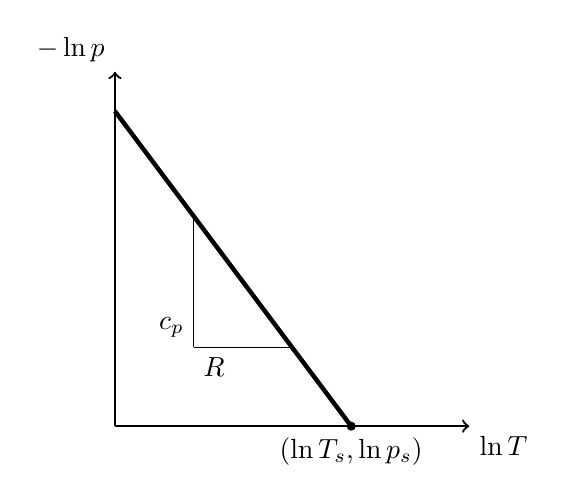
\begin{tikzpicture}
            \draw[thick,->] (0,0) -- (4.5,0) node[anchor=north west] {$\ln T$};
            \draw[thick,->] (0,0) -- (0,4.5) node[anchor=south east] {$-\ln p$};
            \draw[ultra thick] (3,0) node[anchor=north] {$(\ln T_s,\ln p_s)$} -- (0,4);
            \node[circle,draw,fill=black,inner sep=0pt,minimum size =0.1cm] at (3,0){};
            \draw (1,1) node[anchor=north west] {$R$} -- (2.25,1);
            \draw (1,1) node[anchor=south east] {$c_p$} -- (1,2.67);
        \end{tikzpicture}
    \caption{The Dry Adiabat, as predicted by Equation \ref{Dry Adiabat}.}
    \end{subfigure}
    \begin{subfigure}{0.35\linewidth}
        \centering
        \includegraphics[width=0.8\linewidth]{Figures/Thermodynamics/Earth Temperature Profile Radiosonde.png}
    \caption{Radiosonde measurement of Earth's Temperature Profile.}
    \label{Earth T Observation}
    \end{subfigure}
    \caption{The Dry Adiabat: Theory and Observation}
\end{figure}

Note that $R$ and $c_p$ have the same units/dimensions, so $\frac{R}{c_p}$ is dimensionless. We can use the \hyperref[Equipartition]{Equipartition Theorem} to estimate how quickly $T$ falls off with decreasing $p$. We know that $c_v\approx \frac{f}{2}R\approx\frac{5}{2}R$ for the Earth, and we know that $c_p\approx c_v+R$ for an ideal gas. Therefore, $c_p\approx \frac{7}{2}R$, so for the Earth:
\begin{align*}
    \frac{R}{c_p}\approx\frac{R}{\frac{7}{2}R}=\frac{2}{7}\approx\frac{d \ln T}{d \ln p}\approx0.286
\end{align*}

Of course, the atmosphere does not actually follow a \textbf{Dry Adiabat}, as clearly shown by Figure \ref{Earth T Observation}. If we look at only the troposphere (i.e., the lower portion of Figure \ref{Earth T Observation} where $p>\qty{100}{\milli\bar}$), we can estimate from the figure that $d\ln T/d\ln p\approx \frac{\ln(300/180)}{\ln(1000/100)}\approx 0.222$. This is pretty close to the predicted $0.286$, but decidedly much lower! Of course outside of the troposphere our prediction is completely off.

This is because some of our assumptions were not as accurate as we would like. In reality, $dN\neq0$, and entrainment occurs, and $dS\neq0$, and diabatic heating occurs. Some of this diabatic heating is due to condensation, which we will learn how to deal with in the next chapter on \hyperref[Moist Thermodynamics]{Moist Thermodynamics}. We'll find that this will act to shallow the temperature profile (i.e., decrease $d\ln T/d\ln p$). Some of this is radiative heating, which we will discuss in the next part on \hyperref[Radiative Transfer]{Radiative Transfer}.

However, (dry) convection as a mechanism always perturbs an existing atmospheric profile towards an \textbf{Adiabat} and a temperature slope of $2/7$, and it is other processes (radiation, fluid dynamics, moisture) that pull the atmosphere away from an adiabat. In some cases, like in the \textbf{stratosphere}, radiation pulls the atmospheric profile to be super-stable, in which case convection is prohibited due to the stability of the atmosphere. In other cases, these other processes pull the atmospheric profile to be unstable, in which case convection takes over to push the atmosphere back to the \textbf{Adiabat}. What we have just touched upon is \hyperref[Radiative-Convective Equilibrium]{Radiative-Convective Equilibrium}, which we will discuss more in Part \ref{Clouds}.

\section{Potential Temperature}

In basic thermodynamics, we often introduce the concept of temperature operationally in the following way: suppose we have two objects $A$ and $B$, with temperatures $T_A$ and $T_B$, respectively, and we place them in contact with each other. `Temperature' encodes whether heat will flow, and in which way. If $T_A=T_B$, no heat will flow. If $T_B>T_A$, heat will flow from $B$ to $A$, and vice versa if $T_B<T_A$.

However, this will not work in atmospheric thermodynamics. Suppose we have two parcels of air called $A$ and $B$ at pressures $p_A$ and $p_B$\footnote{We are getting used to using pressure as a coordinate rather than height, remember!} with temperatures $T_A$ and $T_B$, respectively. Suppose we displace parcel $A$ in order to place it in contact with parcel $B$ (with no entrainment ($dN=0$) or diabatic heating ($dS=0$)).\vspace{5mm}

Which way will heat flow?\vspace{5mm}

We cannot naively use temperature as we did before, because parcel $A$'s temperature will change following the \hyperref[Dry Adiabat]{Dry Adiabat} as we move it to a different pressure. In other words, temperature is not a variable which is \hyperref[Material Conservation]{Materially Conserved} in Atmospheric/Oceanic Thermodynamics. A variable is \hyperref[Material Conservation]{Materially Conserved} if and only if it remains constant following a air/water parcel. This is a concept which will become very important in Part \ref{Geophysical Fluid Dynamics}.

We now want to define a quantity which serves the same role as temperature did before (i.e., a variable which encodes which way heat will flow) but which is \textit{also}, unlike temperature, \hyperref[Material Conservation]{materially conserved}. Let us consider a more general scenario, and move each parcel to some third pressure $p_{ref}$\footnote{Set $p_{ref}=p_B$ to recover our first example.}. 

We define the \textbf{Potential Temperature} $\theta$ as the temperature a parcel \textit{would} have if it were perfectly adiabatically moved to some reference pressure level $p_{ref}$:
\begin{align}\label{Potential Temperature}
    \BOX{\theta(T,p)=T\left(\frac{p}{p_{ref}}\right)^{-\frac{R}{c_p}}}
\end{align}
Recall that a few pages ago in our derivation of the \hyperref[Dry Adiabat]{Dry Adiabat} we found that:
\begin{align}
    \label{2.5}
    ds=c_p\,d\left(\ln \left(T(p)^\frac{-R}{c_p}\right)\right)
\end{align}

Since the $\ln T(p)^\frac{-R}{c_p}$ term is within the differential, we can freely add and subtract constants within the differential, which corresponds to multiplying within the logarithm.\footnote{
    Another way of looking at this is noting that $d \ln \left(\frac{1}{p_{ref}}\right)^\frac{-R}{c_p}=0$, and so we add $d \ln \left(\frac{1}{p_{ref}}\right)^\frac{-R}{c_p}=0$ to both sides to go from \ref{2.5} to \ref{2.6}.
} We get then that:
\begin{align}
    \label{2.6}
    ds&=c_p\,d\ln T\left(\frac{p}{p_{ref}}\right)^\frac{-R}{c_p}
    \\
    &=c_p\,d\ln\theta
\end{align}

As you can see, if $ds=0$, as we assumed during convection, then $d\theta=0$. Therefore, as we lift or drop a parcel, $\theta$ is \hyperref[Material Conservation]{materially conserved}.\footnote{In the Ocean, even without radiative heating processes, $\theta$ is not conserved. This is because there is a third thermodynamic state variable, salinity, which will change the temperature of sea water without adding any heat. Oceanographers have come up with another kind of materially conserved temperature in the ocean: \textit{Conservative Temperature}.}

Recalling that $TdS=dQ=$ heat, we find that the potential temperature is a measure of the extent to which diabatic/heat transfer processes have heated or cooled our parcel of air. It's essentially a measure of how wrong we were to assume that $dS=0$ in our derivation of \hyperref[Dry Adiabat]{Dry Adiabat}.

\section{Convection}\label{Convection}

\subsection{Buoyancy}

The atmosphere (and ocean) is a fluid, so even in the absence of most forces like friction, gravity is not the only force acting on a fluid parcel. There are also pressure gradient forces, which act to push fluid parcels away from areas of high pressure to areas of low pressure.

We already accounted for the effects of pressure in deriving \hyperref[Hydrostatic Balance]{Hydrostatic Balance} and the \hyperref[Dry Adiabat]{Dry Adiabat}. In the former case, the pressure gradient force acts to push fluid parcels upwards away from lower altitude regions of high pressure to higher altitude regions of low pressure in order to counteract the force of gravity on the ambient air. In the latter case, we only consider large-scale pressure gradients in the ambient atmosphere and we ignored pressure gradients across a fluid parcel.

Now we wish to take into account pressure gradients across a fluid parcel, and consider a fluid parcel which does \textit{not} have the same density as the air around it. Suppose we have a fluid parcel of mass $m$ occupying some volume $V$. For simplicity assume the fluid parcel is rectangular, with a horizontal area of $A$ and a height of $h$ such that $V=Ah$.

Let us consider the forces per unit mass on the fluid parcel in the vertical direction. There are three forces of interest: the gravitational force $F_g=-g$, the pressure force on the \textit{bottom} pushing the parcel \textit{upwards} $F_{bot}=p(z)A/m$, and the pressure force on the \textit{top} pushing the parcel \textit{downards} $F_{top}=p(z+h)A/m$. $p(z)$ is the pressure at height $z$. The net force is then:
\begin{align*}
    F_z=-g-\frac{A}{m}(p(z+h)-p(z))
\end{align*}

We now make two assumptions. First, we assume that $h$ is small, therefore, $p(z+h)-p(z)\approx \frac{dp}{dz} h$. Second, we assume that the pressure in the fluid is set by \hyperref[Hydrostatic Balance]{Hydrostatic Balance}, therefore $p(z+h)-p(z)\approx \frac{dp}{dz} h=-\rho_a g h$, where $\rho_a$ is the density of the ambient air. We define $\rho_p=m/V$ as the density of the fluid parcel, and find that the total force on fluid parcel  is:
\begin{align}
    F_b&=-g+\frac{Ah}{m}\rho_a g\nonumber\\
    &=g\left( -1+ \frac{\rho_a}{\rho_p}\right)\nonumber\\
    \label{Buoyancy Force}
    \therefore \,\,& \BOX{F_b=g\left( \frac{\rho_a-\rho_p}{\rho_p} \right)}
\end{align}
where $F_b=$ the buoyancy force. Physically, the buoyant force is intuitive: if the air parcel is lighter than the ambient air ($\rho_p<\rho_a$) it will convect and rise, and vice versa. Furthermore, we can write $F_b$ in terms of the temperature $T$ (using \ref{Ideal Gas}) or potential temperature $\theta$ (using \ref{Potential Temperature}) in very neat forms, since many terms cancel top and bottom:
\begin{align}
    F_b=g\left( \frac{\rho_a-\rho_p}{\rho_p} \right)\nonumber\\
    \label{Buoyancy Force Temp}
    \boxed{F_b=g\left( \frac{T_p-T_a}{T_a} \right)}\\
    \boxed{F_b=g\left( \frac{\theta_p-\theta_a}{\theta_a} \right)}
\end{align}
So a parcel will convect if it is warmer or has a higher potential temperature than its ambient surroundings.

Finally, another way of thinking of the buoyant force is as a kind of `\textit{reduced gravity}'. The fluid acts like its on a planet of gravitational acceleration $g'=g\left( \frac{\rho_a-\rho_p}{\rho_p} \right)$ not $g$. This will be how we think of things in Chapter \ref{Shallow Water System}. 

\subsection{Convective Instability Criterion}

Now we wish to find whether our atmosphere is convectively stable, i.e., whether the atmosphere will spontaneously undergo convection. If pressure and density did not appreciably change by height, then this would be easy: if $T(z)>T(z+c)$ where $c>0$ (and assuming that $\frac{\partial \rho}{\partial T}<0$), then we will have denser air overlying lighter air, and the parcels will convect.\footnote{
    This is the case if we're considering two layers of different temperature and composition that are in contact. This is because, at the point of contact, pressure changes only infinitessimaly, so the \hyperref[Dry Adiabat]{Dry Adiabat} is inapplicable (since $dp\approx0$). To determine whether these two layers are convectively stable, you must compare the densities directly, which depend on both the temperature of each layer and the molecular composition.
}

As before, the situation is a bit more complicated in an atmosphere when density and pressure vary significantly with height. Suppose again that we have an atmospheric temperature profile $T=T(p)$ (not necessarily following the dry adiabat). Suppose we lift a parcel at some pressure $p$ to some (smaller) pressure $p-\delta p$.

That parcel will be convectively unstable and continue rising if it is lighter (and therefore hotter) than the ambient surrounding air. We assume that the parcel is initially in equilibrium with its surroundings ($T_{parcel}(p)=T_{ambient}(p)$). We then Taylor Expand:
\begin{align*}
    T_{parcel}(p-\delta p)&>T_{ambient}(p-\delta p)\\
    {T_{parcel}(p)}-\frac{d T_{parcel}}{d p}\delta p & >T_{ambient}(p)-\frac{d T_{ambient}}{d p}\delta p\\
    \frac{d \ln T_{parcel}}{d \ln p} & <\frac{d \ln T_{ambient}}{d \ln p}
\end{align*}
Substituting in the \hyperref[Dry Adiabat]{Dry Adiabat} for $\frac{d \ln T_{parcel}}{d \ln p}$ we find the dry stability criterion:
\begin{fact}{The Dry Stability Criterion}{Dry Stability Box}\label{Dry Stability Box}
Suppose a dry atmosphere has a temperature profile $T(p)$. It will be:
\begin{multicols}{3}
    \centering
    Unstable to convection if:\newline
    \begin{align}\label{Dry Stability}
        \BOX{\frac{d\ln T}{d\ln p}>\frac{R}{c_p}}
    \end{align}
    Neutrally stable to convection if:
    \begin{align}
        \BOX{\frac{d\ln T}{d\ln p}=\frac{R}{c_p}}
    \end{align}
    and Stable to convection if:
    \begin{align}\label{Dry Stability Stable}
        \BOX{\frac{d\ln T}{d\ln p}<\frac{R}{c_p}}
    \end{align}
\end{multicols}
\end{fact}
Note that \ref{Dry Stability} and \ref{Dry Stability Stable} are not automatically ruled out due to \ref{Dry Adiabat}. That is because \ref{Dry Adiabat} governs a perfectly adiabatic rising/falling parcel of air. While this is the dominant contribution to the atmospheric temperature profile in the troposphere,  it is not the only one (even within the troposphere). Other processes (water vapour, radiation, dynamics) can push the atmospheric temperature profile away from the dry adiabat and make it stable or unstable. However, typically, unstable atmospheres are removed very quickly through spontaneous convection.

Physically, the idea is as follows: an atmosphere is stable if the temperature decreases slow enough with height (\ref{Dry Stability Stable}). If it decreases too quickly (\ref{Dry Stability}), a lifted parcel of air will have cooled \textit{less} than its surroundings, and thus be warmer and lighter than its surroundings, and continue to rise due to buoyancy (\ref{Buoyancy Force Temp}).

If \ref{Dry Stability Stable} obtains then an atmosphere will be \textit{super-stable} and will inhibit convection. A quick sanity check to remember which way the inequality is in \ref{Dry Stability Stable} is the following: an isothermal\footnote{
    `Iso' meaning same and `thermal' meaning temperature, so `Isothermal' means constant temperature.
} atmosphere is always super-stable. An isothermal atmosphere will have $\frac{d \ln T}{d \ln p} = 0$, so $\left( \frac{d \ln T}{d \ln p} < \frac{R}{c_p} \right)$ corresponds to stability. If one has a \textit{super-stable} atmosphere then that indicates that there has been some other dominant energy transport mechanism that has kept the atmosphere in this state. This is characteristic of a \textbf{stratosphere}.\footnote{
    Recall the footnote on \hyperref[Vertical Structure]{this} page. This is why Ray prefers that definition of \textbf{stratosphere}: a stratsophere should be characterised by what energy transport mechanism is dominant, not whether it happens to have shortwave absorbers.
} 

\begin{figure}[H]
    \centering
    \begin{tikzpicture}
        \begin{scope}
            \draw[thick,->] (0,0) -- (4,0) node[anchor=south] {$\ln T$};
            \draw[thick,->] (0,0) -- (0,4) node[anchor=south east] {$-\ln p$};
            \draw[ultra thick] (3,0) node[anchor=north] {$(\ln T_s,\ln p_s)$} -- (0,3);
            %\draw[ultra thick] (3,0) node[anchor=north] {$(\ln T_s,\ln p_s)$} -- (0,4);
            \node[circle,draw,fill=black,inner sep=0pt,minimum size =0.1cm] at (3,0){};
            \node[circle,draw,fill=mymagenta,inner sep=0pt,minimum size =0.2cm] (A) at (1.5,1.5){};
            \node at (2.5,2.5){Unstable};
            \node[] (B) at (2.4,0.3){};
            \node[] (C) at (0.6,2.7){};
            \draw[thick,mymagenta] (B) -- (C);
        \end{scope}
        \begin{scope}[xshift=5.5cm]
            \draw[thick,->] (0,0) -- (4,0) node[anchor=south] {$\ln T$};
            \draw[thick,->] (0,0) -- (0,4) node[anchor=south east] {$-\ln p$};
            \draw[ultra thick] (2.625,0) node[anchor=north] {$(\ln T_s,\ln p_s)$} -- (0,3.5);
            %\draw[ultra thick] (3,0) node[anchor=north] {$(\ln T_s,\ln p_s)$} -- (0,4);
            \node[circle,draw,fill=black,inner sep=0pt,minimum size =0.1cm] at (2.625,0){};
            \node[circle,draw,fill=mymagenta,inner sep=0pt,minimum size =0.2cm] (A) at (1.5,1.5){};
            \node at (2.5,2.5){Neutrally Stable};
            \node[] (B) at (2.4,0.3){};
            \node[] (C) at (0.6,2.7){};
            \draw[thick,mymagenta] (B) -- (C);
        \end{scope}
        \begin{scope}[xshift=11cm]
            \draw[thick,->] (0,0) -- (4,0) node[anchor=south] {$\ln T$};
            \draw[thick,->] (0,0) -- (0,4) node[anchor=south east] {$-\ln p$};
            \draw[ultra thick] (1.5,0) node[anchor=north] {$(\ln T_s,\ln p_s)$} -- (1.5,3);
            %\draw[ultra thick] (3,0) node[anchor=north] {$(\ln T_s,\ln p_s)$} -- (0,4);
            \node[circle,draw,fill=black,inner sep=0pt,minimum size =0.1cm] at (1.5,0){};
            \node[circle,draw,fill=mymagenta,inner sep=0pt,minimum size =0.2cm] (A) at (1.5,1.5){};
            \node at (2.5,2.5){Stable};
            \node[] (B) at (2.4,0.3){};
            \node[] (C) at (0.6,2.7){};
            \draw[thick,mymagenta] (B) -- (C);
        \end{scope}
    \end{tikzpicture}
    \caption{Dry Stability: From left to right: unstable, neutrally stable, and super stable atmospheric temperature profiles. Thick black is the atmospheric profile, thin magenta is the dry adiabatic slope.}
\end{figure}

\subsection{Convective Stability Criterion with Potential Temperature}

We can formulate an equivalent criterion for potential temperature. Recall that if two parcels of air have potential temperatures $\theta_A$ and $\theta_B$ such that $\theta_A>\theta_B$, then parcel $A$ will have a higher temperature than parcel $B$ if they're at the same pressure.

We can very straightforwardly derive an equivalent criterion for convective instability, this time in terms of potential tempreature $\theta$, by rearranging \ref{Potential Temperature} for $T(\theta)$ and substituting that into \ref{Dry Stability}.

\begin{align*}
    1&<\frac{c_p}{R}\frac{d\ln T(\theta)}{d\ln p}
    &\text{ ; }&\text{\ref{Dry Stability}}
    \\
    &=\frac{c_p}{R}\frac{d\ln \left( \theta\left( \frac{p}{p_{ref}} \right)^{\frac{R}{c_p}} \right)}{d\ln p}
    &\text{ ; }&\text{substitute \ref{Potential Temperature}}
    \\
    &=\frac{c_p}{R} \left( 
        \frac{d \ln \theta}{d \ln p}+
        \frac{d \ln \left(p^{\frac{R}{c_p}} \right)}{d \ln p}+
        \frac{d \ln \left(p_{ref}^{\frac{-R}{c_p}} \right)}{d \ln p}
     \right)
    &\text{ ; }&\text{split logarithm}
    \\
    &=\frac{c_p}{R}\frac{p}{\theta}\frac{d\theta}{dp}+\frac{c_p}{R}\frac{R}{c_p}
    &\text{ ; }
    &\ln p^{R/c_p}=R/c_p\ln p
\end{align*}
Therefore, since $\theta>0$ and $p>0$ always, we get that our atmosphere is unstable if and only if:
\begin{align}\label{Dry Stability Potential Temperature}
    \boxed{\frac{d\theta}{dp}>0}
\end{align}
Using the hydrostatic relation and the fact that $g>0,\rho>0$, we get our criterion for instability in height coordinates:
\begin{align}
    \BOX{\frac{d\theta}{dz}<0}
\end{align}

Therefore, if potential temperature decreases with height, then our atmosphere is unstable. This makes physical sense. Recall that potential temperature takes the place of temperature in atmospheric thermodynamics in the sense that it is \textit{potential temperature} that stays the same when you lift/drop and air parcel. If you lift an air parcel, its potential temperature stays the same. However, if the ambient potential temperature decreases with height, then it will be colder than the air parcel, and the air parcel will keep rising.

\begin{figure}[H]
    \centering
    \begin{tikzpicture}
        \begin{scope}
            \draw[thick,->] (0,0) -- (4,0) node[anchor=south] {$\theta$};
            \draw[thick,->] (0,0) -- (0,4) node[anchor=south east] {$z$};
            \draw[ultra thick] (3,0) node[anchor=north] {$(\theta_s,0)$} -- (0,3);
            %\draw[ultra thick] (3,0) node[anchor=north] {$(\ln T_s,\ln p_s)$} -- (0,4);
            \node[circle,draw,fill=black,inner sep=0pt,minimum size =0.1cm] at (3,0){};
            \node[circle,draw,fill=mymagenta,inner sep=0pt,minimum size =0.2cm] (A) at (1.5,1.5){};
            \node at (2.5,3.5){Unstable};
            \node[] (B) at (1.5,0.3){};
            \node[] (C) at (1.5,2.7){};
            \draw[thick,mymagenta] (B) -- (C);
        \end{scope}
        \begin{scope}[xshift=5.5cm]
            \draw[thick,->] (0,0) -- (4,0) node[anchor=south] {$\theta$};
            \draw[thick,->] (0,0) -- (0,4) node[anchor=south east] {$z$};
            \draw[ultra thick] (1.5,0) node[anchor=north] {$(\theta_s,0)$} -- (1.5,3);
            %\draw[ultra thick] (3,0) node[anchor=north] {$(\ln T_s,\ln p_s)$} -- (0,4);
            \node[circle,draw,fill=black,inner sep=0pt,minimum size =0.1cm] at (1.5,0){};
            \node[circle,draw,fill=mymagenta,inner sep=0pt,minimum size =0.2cm] (A) at (1.5,1.5){};
            \node at (2.5,3.5){Neutrally Stable};
            \node[] (B) at (1.5,0.3){};
            \node[] (C) at (1.5,2.7){};
            \draw[thick,mymagenta] (B) -- (C);
        \end{scope}
        \begin{scope}[xshift=11cm]
            \draw[thick,->] (0,0) -- (4,0) node[anchor=south] {$\theta$};
            \draw[thick,->] (0,0) -- (0,4) node[anchor=south east] {$z$};
            \draw[ultra thick] (0,0) node[anchor=north west] {$(\theta_s,0)$} -- (3,3);
            %\draw[ultra thick] (3,0) node[anchor=north] {$(\ln T_s,\ln p_s)$} -- (0,4);
            \node[circle,draw,fill=black,inner sep=0pt,minimum size =0.1cm] at (0,0){};
            \node[circle,draw,fill=mymagenta,inner sep=0pt,minimum size =0.2cm] (A) at (1.5,1.5){};
            \node at (2.5,3.5){Stable};
            \node[] (B) at (1.5,0.3){};
            \node[] (C) at (1.5,2.7){};
            \draw[thick,mymagenta] (B) -- (C);
        \end{scope}
    \end{tikzpicture}
    \caption{Dry Stability: From left to right: unstable, neutrally stable, and super stable atmospheric temperature profiles. Thick black is the atmospheric profile, thin magenta is the dry adiabatic slope.}
\end{figure}

\subsection{CAPE, LFC, LNB}

We have so far characterised \textit{whether} convection will occur in our dry atmosphere, but now we wish to know what will happen \textit{during} convection. We start again by considering a parcel of air at an initial pressure $p_0$ with a temperature of $T_p(p_0)$. Let $T_a(p)$ be the temperature profile of the ambient atmosphere, and assume that initially the parcel is in equilibrium with its surroundings (i.e., assume $T_p(p_0)=T_a(p_0)$).

We define the \textbf{L}evel of \textbf{F}ree \textbf{C}onvection (\textbf{LFC}) $p_{LFC}$ as the \textit{closest} location to $p_0$ where $T_p(p)=T_a(p)$, $dT_p/dp<dT_a/dp$ (the parcel is convectively unstable), and $p<p_0$ (it's higher). 

We define the \textbf{L}evel of \textbf{N}eutral \textbf{B}uoyancy (\textbf{LNB}) $p_{LNB}$ as the location where $T_p(p)=T_a(p)$, $dT_p/dp>dT_a/dp$ (the parcel is convectively stable), and $p<p_{LFC}$ (it's higher than the \textbf{LFC}).

We define the \textbf{C}onvective \textbf{A}vailable \textbf{P}otential \textbf{E}nergy (\textbf{CAPE}) as the total available potential energy (per unit mass) for a parcel of air from the Level of Free Convection to the Level of Neutral Buoyancy. In other words, $CAPE$ is equal to the total kinetic energy per unit mass a parcel would gain if it was allowed to convect from the Level of Free Convection to the Level of Neutral Buoyancy:
\begin{align}
    CAPE=\int_{z_{LFC}}^{z_{LNB}}F_b\,dz
\end{align}
We can substitute for $F_b$ using \ref{Buoyancy Force Temp} and convert to pressure coordinates using \ref{Hydrostatic Balance Ideal} to find that:
\begin{gather*}
    CAPE=\int_{z_{LFC}}^{z_{LNB}}\frac{T_p-T_a}{T_a}g\,dz\\
    =\int_{p_{LFC}}^{p_{LNB}}\frac{T_p-T_a}{\bcancel{T_a}}(-R\bcancel{T_a}\,d\ln p)\\
    \therefore \boxed{CAPE=R\int_{p_{LNB}}^{p_{LFC}}\left( T_p-T_a \right)\,d\ln p}
\end{gather*}
We know $T_p(p)$, since $T_p(p)$ follows the \hyperref[Dry Adiabat]{Dry Adiabat} with $(p_0,T_0)=(p_{LFC},T_{LFC})$, so we can straightfowardly calculate $CAPE$ if we are given the atmospheric temperature profile $T_a(p)$.

We further define \textbf{C}onvective \textbf{IN}hibition (\textbf{CIN}) as the energy a fluid parcel would need to overcome to reach the \textbf{LFC}:
\begin{align*}
    \boxed{CIN = R\int_{p_{LFC}}^{p_{0}}\left( T_p-T_a \right)\,d\ln p}
\end{align*}
We expect $CIN<0$ and $CAPE>0$. Above \textbf{LNB}, we expect there to be more `$CIN$', which will prevent the parcel from rising further. However, at this point, the parcel will have already gained kinetic energy from $CAPE$. We call where the parcel `stops' the \textbf{L}evel of \textbf{M}aximum \textbf{A}scent (\textbf{LMA}), which occurs at $p_{LMA}$ where the `$CIN$' above \textbf{LNB} equals the $CAPE$:
\begin{align*}
    \boxed{
        R\int_{p_{LMA}}^{p_{LNB}}\left( T_p-T_a \right)\,d\ln p = 
        R\int_{p_{LNB}}^{p_{LFC}}\left( T_p-T_a \right)\,d\ln p
    }
\end{align*}

\begin{fact}{Convection Definitions}{Convection Box}\label{Convection Box}
    Let the ambient air temperature be $T_a(p)$ (black line \textcolor{black}{\rule{0.25cm}{0.25cm}}). Consider an air parcel at an initial pressure $p_0$ with a temperature of $T_p(p_0)=T_a(p_0)$ that is then lifted. Upon lifting, the parcel's temperature $T_p(p)$ follows the \hyperref[Dry Adiabat]{Dry Adiabat} (\textcolor{mymagenta}{dashed magenta line \rule{0.25cm}{0.25cm}}). Then:
    \begin{quote}
        \textbf{Level of Free Convection} (\textbf{LFC}): $p=p_{LFC}$ if $T_p(p)=T_a(p)$, $dT_p/dp<dT_a/dp$, and this is the first pressure $p<p_0$ where this occurs.

        \textbf{Level of Neutral Buoyancy} (\textbf{LNB}): $p=p_{LNB}$ if $T_p(p)=T_a(p)$, $dT_p/dp>dT_a/dp$, and this is the first pressure $p<p_{LFC}$ where this occurs.

        \textbf{Level of Maximum Ascent} (\textbf{LMA}): $p=p_{LMA}$ where $p_{LMA}$ is determined by Equation \ref{LMA} (I.e., where the blue area \textcolor{mydarkblue}{\rule{0.25cm}{0.25cm}} equals the orange area \textcolor{myorange}{\rule{0.25cm}{0.25cm}}).
    \end{quote}

    \noindent\begin{minipage}{.48\linewidth}
        \begin{align}
        \label{CAPE}
        \BOX{CAPE=R\int_{p_{LNB}}^{p_{LFC}}\left( T_p-T_a \right)\,d\ln p}\\
        \label{CIN}
        \BOX{CIN=R\int_{p_{LFC}}^{p_{0}}\left( T_p-T_a \right)\,d\ln p}\\
        \label{LMA}
        \BOX{R\int_{p_{LMA}}^{p_{LNB}}\left( T_p-T_a \right)\,d\ln p = CAPE}
    \end{align}
    \end{minipage}
    \hspace{5mm}
    \begin{minipage}{.48\linewidth}
    \begin{figure}[H]
        \centering
        \begin{tikzpicture}
            \draw[->] (0,0) -- (4.5,0) node[anchor=west]{$T$};
            \draw[->] (0,0) -- (0,4.5) node[anchor=south]{$-\ln p$};
            \coordinate (ps) at (4.2,0);
            \node[] at (4.2,-0.4) {$p_s$};
            \coordinate (p0) at (4,0.5);
            \node[] at (4.35,0.5) {$p_0$};
            \coordinate (end) at (0,4.5);
            \coordinate (LFC) at (2.7,1.8);
            \node[] at (3.1,2.1) {\textbf{LFC}};
            \node[] at (2.7,1) {$CIN$ \textcolor{myyellow}{\rule{0.25cm}{0.25cm}}};
            \coordinate (LNB) at (1.3,3.2);
            \node[] at (0.8,3) {\textbf{LNB}};
            \coordinate (LMA) at (0.8,4.5);
            \node[] at (1.6,4.5) {\textbf{LMA}};
            \node[] at (2.7,2.8) {$CAPE$ \textcolor{mydarkblue}{\rule{0.25cm}{0.25cm}}};
            \filldraw[thick,fill=myyellow] (p0) .. controls +(0,1) and +(1,0) .. (LFC);
            \filldraw[thick,fill=mydarkblue] (LFC) .. controls +(-1,0) and +(0,-1) .. (LNB);
            \path[fill=myorange] (LNB) .. controls +(0,0.5) and +(0.5,-0.5) .. (LMA) -- (end);
            \draw[dashed,mymagenta,thick] (p0) -- (end);
            \node[circle,draw,fill=black,inner sep=0pt,minimum size =0.15cm] at (ps){};
            \node[circle,draw,fill=black,inner sep=0pt,minimum size =0.15cm] at (p0){};
            \node[circle,draw,fill=black,inner sep=0pt,minimum size =0.15cm] at (LFC){};
            \node[circle,draw,fill=black,inner sep=0pt,minimum size =0.15cm] at (LNB){};
            \node[circle,draw,fill=black,inner sep=0pt,minimum size =0.15cm] at (LMA){};
            \draw[thick] (ps) .. controls +(0,0.1) and +(0,-0.5) .. (p0);
            \draw[thick] (LNB) .. controls +(0,0.5) and +(0.5,-0.5) .. (LMA);
        \end{tikzpicture}
        \caption{Atmospheric Profile. The parcel is lifted from $p_0$. $CIN$ is proportional to the area shaded in \textbf{\textcolor{myyellow}{Yellow \rule{0.25cm}{0.25cm}}} and $CAPE$ is proportional to the area shaded in \textcolor{mydarkblue}{\textbf{Blue} \rule{0.25cm}{0.25cm}}.}
    \end{figure}
    \end{minipage}
\end{fact}

\subsection{Conservation of Enthalpy during Convection}

We define the (specific) \textbf{Enthalpy} $h$ as follows:
\begin{align}
    h=u+p\frac{1}{\rho}
\end{align}
For an ideal gas, we can substitute for $p$ using \ref{Ideal Gas} and $u=c_vT$ to write $h$ in terms of $T$ only:
\begin{align*}
    h&=\underbrace{c_vT}_{u}+\underbrace{\rho R T}_{p}\frac{1}{\rho}\\
    &=\underbrace{(c_v+R)}_{c_p}T\\
    &=c_pT
\end{align*}
Therefore we can interpret the enthalpy $h$ as an expression of the heat content of a system at constant pressure, like for example in the atmosphere.

We introduce the enthalpy because we can show that, under suitable assumptions, the total enthalpy $H$ of an atmospheric column is conserved during convection:
\begin{align*}
    H=\iiint \rho h\,dV=const
\end{align*}
We make three assumptions:
\begin{enumerate}
    \item The initial and final states are both in Hydrostatic Balance \ref{Hydrostatic Balance}
    \item The kinetic energy of the initial and final state is negligible compared to the potential and internal energy.
    \item No mass or heat leaves domain.
\end{enumerate}
The last assumption requires some elaboration. First, we \textit{don't} assume that no energy leaves the domain: we allow the column to do work on the air above or below itself as it expands/contracts. Second, we \textit{don't} assume that there is no heating within the column. In fact, we expect there to be some heating within the column in general: If a column is convectively unstable, then there will be \textbf{CAPE}, and we expect this to be converted into an appreciable amount of kinetic energy as the air parcels within the column convect. Once convection acts to remove the \textbf{CAPE}, we expect friction to slow the parcels down and convert the kinetic energy into heat. 

We first consider the total energy in an atmospheric column per horizontal area between altitudes $z_0$ and $z_1$, which is the sum of the internal energy $u$ and the potential energy $gz$ (and we have assumed kinetic energy $\frac{1}{2}v^2$ is negligible):
\begin{align*}
    E &= \int_{z_0}^{z_1} \rho \left( u + gz \right)dz\\
    &=\frac{1}{g}\int_{p_1}^{p_0} \left( u+gz \right)dp
\end{align*}
We then integrate the potential energy term $gz$ by parts:
\begin{align*}
    g\int_{p_1}^{p_0} z\,dp &= g\left[ zp \right]_{p_0}^{p_1}-g\int_{z_1}^{z_0}p\,dz\\
    &=g(z_0p_0-z_1p_1)+\int_{p_1}^{p_0}\frac{p}{\rho}dp
\end{align*}
Therefore the total energy per unit area is:
\begin{align*}
    E=\frac{1}{g}\int_{p_1}^{p_0}\left(u+\frac{p}{\rho} \right)\,dp+(z_0p_0-z_1p_1)
\end{align*}
We make a final, fourth assumption here that the pressure at the bottom $p_0$ and top $p_1$ of the column is unchanged between the final and initial states. This is ensured if we assume the entire column (inside and outside the column under consideration) is in hydrostatic balance and the mass of the air above, within, and below the column under consideration is unchanged (recall \ref{Hydrostatic Differential}). The change in energy $\Delta E$ between the final and initial states is then:
\begin{align}
    \label{Delta E 1}
    \Delta E = \frac{1}{g}\Delta \int_{p_1}^{p_0}h\,dp + p_0 \Delta z_0 - p_1 \Delta z_1
\end{align}
We now wish to equate this with the change in energy of the atmospheric column governed by \ref{First Law}. Since we have assumed that there is no heat or mass transfer to or from the system, we can set $dN=0$ and approximate $dS=0$. Therefore, the change in energy (per unit area), to a good approximation, is set by:
\begin{align}
    dE &= -p\,dV/A\nonumber\\
    &=p_0 d z_0-p_1 d z_1\nonumber\\
    \label{Delta E 2}
    \therefore \Delta E & = p_0 \Delta z_0 - p_1 \Delta z_1 
\end{align}
Therefore, setting \ref{Delta E 1} equal to \ref{Delta E 2} we can cancel the $p\Delta z$ to find that:
\begin{align}
    \BOX{\Delta H = \Delta \iiint \rho h \,dz\,dx\,dy=0}
\end{align}
The enthalpy of a column is conserved under convection. If we assume that the atmosphere is an ideal gas (so that $h=c_pT$) and that $c_p$ is approximately independent of temperature (so that we can pull $c_p$ out of the integral), then we can convert to pressure coordinates to find that:
\begin{align*}
    H =  \int \int \frac{c_p}{g} \int  T \,dp\,dx\,dy
\end{align*}
Therefore we find that the enthalpy is proportional to $\int T\,dp$, and so:
\begin{align}
    \boxed{
        \Delta \int T dp = 0
    }
\end{align}
during convection.

\chapter{Moist Thermodynamics}\label{Moist Thermodynamics}

\section{Phase Transitions}

In the previous chapter, we considered only atmospheres made up completely of constituents that do not undergo any phase transitions. However, Earth's atmosphere (and many others) clearly do not obey this assumption. Earth's atmosphere has a non-negligible amount of condensible substances: water vapour (look outside and you might see a cloud!), which clearly condense, evaporate, and freeze in Earth-like conditions.

So what is a phase transition? We will only be dealing with what are called \textbf{First-Order Phase Transitions}, which occur when there is a \textit{discontinuity} in a thermodynamic state variable and an absorption or release of a large amount of energy, called \textbf{latent heat}. Phase transitions occur at certain temperatures and pressures\footnote{Whether a phase transition will occur might also depend on other thermodynamic state variables. For example, salinity is a thermodynamic variable which affects when sea water evaporates/freezes.}. We can represent this with a \textbf{Phase Diagramme}, as shown below:

\begin{figure}[H]
    \centering
    \begin{subfigure}{0.45\linewidth}
        \centering
        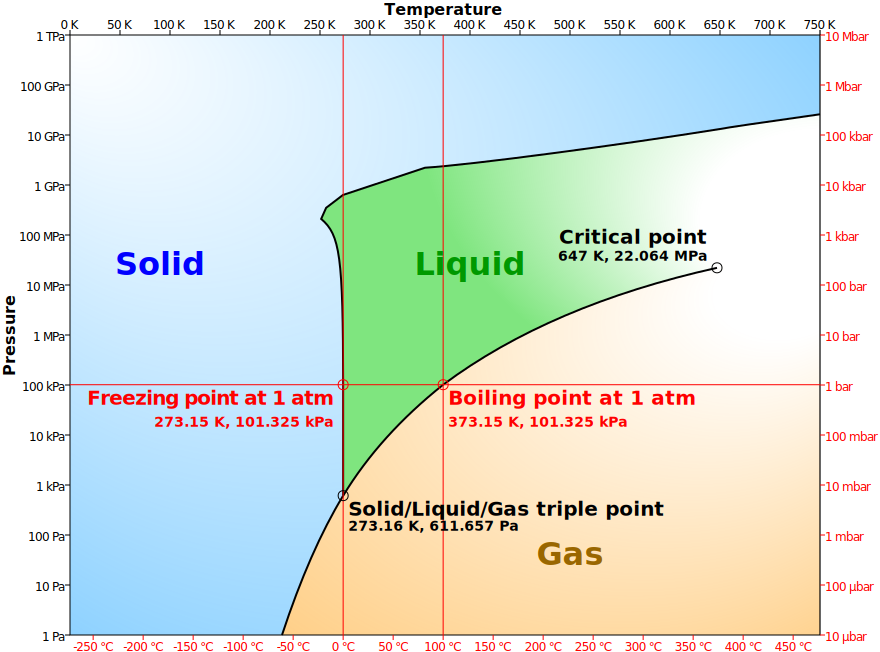
\includegraphics[width=\linewidth]{Figures/Thermodynamics/Phase_diagram_of_water_simplified.svg.png}
    \end{subfigure}
    \begin{subfigure}{0.45\linewidth}
        \centering
        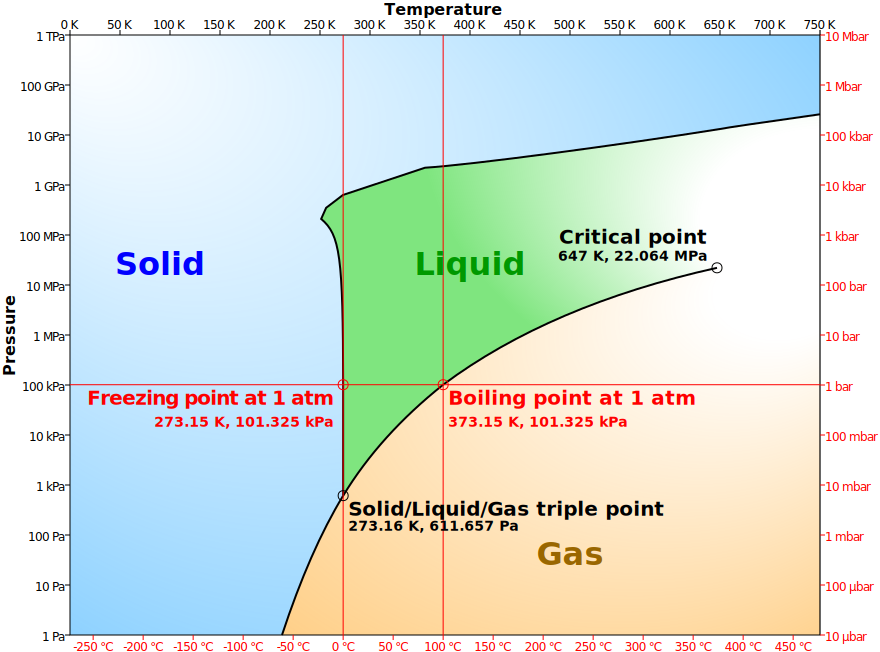
\includegraphics[width=\linewidth]{Figures/Thermodynamics/Phase_diagram_of_water_simplified.png}
    \end{subfigure}
    %\includesvg{Figures/Thermodynamics/Phase_diagram_of_water_simplified}
    \caption{Phase Diagramme for Water from Wikipedia \cite{PhaseDiagramme}.}
    \label{Phase Diagramme}
\end{figure}

Focus on the left-hand plot for now. The coloured regions indicate what phase water will be in at a certain the partial pressure (of the water) and temperature: gas (vapour), liquid (steam), and solid (ice). Crucially, this does not depend on the total pressure of the atmosphere or surrounding gases, but only the partial pressure of the condensible substance (in this case, the partial pressure of water). The solid black lines indicate \textbf{Phase Boundaries}. The \textbf{Triple Point} is the point where all three states can coexist. The \textbf{Critical Point} is the point past which there is no phase transition between gas and liquid.

The pressure at the \textbf{Phase Boundaries} is the \textbf{Saturation Vapour Pressure} $p_{sat}(T)$. If the partial pressure $p<p_{sat}$, then more vapour (gas form) can be added without condensing. If the $p\geq p_{sat}$, then the gas will condense until the partial pressure reaches the saturation vapour pressure. However, it's important to remember that condensation is not instantaneous, which is partly why we can have atmospheric conditions where $p>p_{sat}$. This will be important when we consider \hyperref[Clouds]{Clouds}.

In fact all gases can condense if the temperature is low enough/partial pressure is high enough. CO$_2$ condenses on Mars, and N$_2$ condenses on Neptune. Why doesn't CO$_2$ and N$_2$ condense here on Earth? It all depends on the vertical structure of the atmosphere: the precise profile of $T=T(p)$. Recall that, as $p$ decreases, so too does $T$ (if our atmosphere follows the \hyperref[Dry Adiabat]{Dry Adiabat}). There are three cases, all labeled in the right-hand plot of Figure \ref{Phase Diagramme}.

\begin{enumerate}
    \item Case 1: The atmosphere has such a high pressure/temperature that it avoids a phase transition altogether by meandering around the critical point.
    \item Case 2: The atmospheric profile cuts right through a phase boundary, and the condensible condenses (clouds form!).
    \item Case 3: The stratosphere starts before the atmosphere hits the phase boundary, in which case temperature no longer decreases with height, so it never crosses the phase boundary.
\end{enumerate}

For O$_2$ and N$_2$ in Earth like conditions, we are in case 3: it never gets cold enough for O$_2$ and N$_2$ to condense, which is why we have no O$_2$ and N$_2$ clouds. However, we are in Case 2 with water (H$_2$O), and so we do get water clouds!

When a gase condenses from phase $A$ to phase $B$, it typically releases a large amount of \textbf{Latent Heat}. Again, we would like to work in intensive variables, so we often work with the \textbf{Specific Latent Heat} $L_{A\to B}$ (units of \qty{}{\joule\per\kilogram}) which is the amount of energy released per kilogram of substance when underoing a phase transition from $A$ to $B$ ($L_{A\to B}>0$ if heat is released). Like heat capacity, this often has a temperature dependence, but we will in most cases treat this as constant.

\section{The Clausius-Clapeyron Relation}

We can derive the shape of the phase boundary with the \textbf{Clausius Clapeyron Relation}, which relates the saturation vapour pressure to the temperature using the latent heat and the densities. We will not derive it here, but it would be useful for you to memorise the following relation:
\begin{align}\label{Clausius Clapeyron}
    \BOX{
        \frac{dp_{sat}}{dT}=\frac{L_{A\to B}}{T\left(\frac{1}{\rho_A}-\frac{1}{\rho_B}\right)}
        }
\end{align}
If we assume that $\rho_g\ll\rho_l$ (i.e., the gaseous form is much less dense than the liquid form), and that the gas is ideal, we find that:
\begin{align}
    \frac{d p_{sat}}{dT}&\approx\frac{L_{g\to l}}{T \frac{1}{\rho_g}}\nonumber\\
    & = \frac{L_{g \to l} p}{R_cT^2}\nonumber\\
    \therefore \,\,\,& \boxed{\frac{d \ln p_{sat}}{d \left( \frac{1}{T} \right)} \approx -\frac{L_{g\to l}}{R_c}}\label{Clausius Clapeyron Simplified}
\end{align}

Note that I have written $R_c$ to make clear that $R_c$ is the specific gas constant for the condensible (e.g., water) \textit{not} for the atmosphere. We can now derive an analytic expression for the saturation vapour pressure if we further assume that the latent heat is constant. 
\begin{align}
    \boxed{
        p_{sat}\approx p_0 \,e^{\frac{L}{R_c}\left( \frac{1}{T_0}-\frac{1}{T} \right)}
    }
    \label{Sat Vap Pressure}
\end{align}
where I now just write $L$ for the latent heat of condensation and $(T_0,p_0)$ are any point on the saturation vapour pressure curve. This could be, for example, the \textbf{triple point} or the \textbf{critical point}.

As we can see then, the saturation vapour pressure depends approximately \textit{exponentially} on temperature, so saturation vapour pressure decreases exponentially as temperature decreases. Conversely, if saturation vapour pressure decreases, T changes only logarithmically (i.e., very slowly).

\section{The Moist Pseudo-Adiabat: Lifting Moist Parcels of Air}\label{Moist Pseudo Adiabat}

Our goal now is to derive an analogous \hyperref[Dry Adiabat]{Dry Adiabat} relation for moist atmospheres consisting of some condensible substance $c$. We call this the \textbf{Moist Pseudo-Adiabat}. We call this a `\textit{Pseudo}'-Adiabat because we assume, for mathematical convenience, that the condensible substance $c$ is instantaneously removed from the air parcel. This occurs if, for example, $c$ instantaneously rains out (but rain is not the only way in which this may occur!). When the condensible is removed, this constitutes a diabatic process ($dN\neq 0$), so strictly speaking we will not derive an adiabat in this section.

In reality, rising moist air parcels that condense will not instantaneously eject its condensed $c$, and so will not follow the pseudo-adiabat. However, the pseudo-adiabat is a good approximation if the amount of condensate left in the air parcel is small, which is at least the case on Earth.

Recall that we are using the same logic as we did before in deriving the \hyperref[Dry Adiabat]{Dry Adiabat}. As such, we are still assuming that the dominant mechanism of heat transport within the atmosphere is vertical convection, only this time the air parcels convecting are moist (have condensible substances in them). 

We will now consider two limiting cases. In both cases, we make the crucial assumption that the air parcels remain saturated with the condensible. In other words, we assume that the partial pressure of the condensible is equal to the saturation vapour pressure $p_{sat}$.

\subsection{Limit I: Single Component Condensible Atmosphere} 

We consider the first limiting case, with an atmosphere made up wholly of one condensible substance $c$. Since there is only one constituent, the total pressure is equal to the partial pressure of the $c$. There are two possibilities now.

The first possibility obtains if the temperature at the ground $T_g(p_g)$ is too low such that $p_g>p_{sat}(T_g(p_g))$, i.e., the pressure at the ground is higher than the saturation vapour pressure at the ground. Then there will be an ocean of $c$ at the surface. The pressure within the ocean will obey \hyperref[Hydrostatic Balance]{Hydrostatic Relation}, and the surface of the ocean is determined by where the pressure and temperature intersect the phase boundary ($p=p_s=p_{sat}(T_s(p_s))$).

The temperature above the surface of the ocean is set by convecting air parcels. These air parcels originate from the surface of the ocean, and are initially saturated. However, recall that we have assumed that the air parcel remains saturated.\footnote{
    I'm not sure how justified this assumption is. I plan to ask Ray about this at some point, but if this footnote is still here when you're reading it I have not (yet).
} As such, the atmospheric profile must lie on the phase boundary, so the temperature is fixed to the phase boundary and is as follows (found by rearranging \ref{Sat Vap Pressure} for $T$ in terms of $p_{sat}$):
\begin{align}
    \text{If } p_g>p_{sat(T_g)}\text{: }& T(p)=\frac{T_s}{1-\frac{RT_s}{L}\ln\frac{p}{p_{s}}} \label{1 component moist adiabat} \\
    &p_s = p_{sat}(T_s)
\end{align}

The surface pressure $p_s$, then, is set by the surface temperature $T_s$. Recalling Equation \ref{Total Mass Hydrostatic}, the mass of the atmosphere is set by how hot it is. Physically, this corresponds to how much $c$ you can evaporate from the ocean!

The second possibility obtains if the temperature at the ground $T_g(p_g)$ is too high such that $p_g<p_{sat}(T_g(p_g))$, i.e., the pressure at the ground is lower than the saturation vapour pressure at the ground. Then there will be no surface $c$ ocean, and the  atmosphere will follow the \hyperref[Dry Adiabat]{Dry Adiabat} until it reaches the phase boundary at the \textbf{lifted condensation level}, after which it will follow Equation \ref{1 component moist adiabat}:
\begin{align}
    \text{If } p_s<p_{sat(T_s)}\text{: }
    &
    T(p)=
    \begin{cases}
        T_s\left(\frac{p}{p_s}\right)^\frac{R}{c_p} \text{ for }p<p_{LCL}\\
        \frac{T_s}{1-\frac{RT_s}{L}\ln\frac{p}{p_{LCL}}}, \text{ for }p>p_{LCL}
    \end{cases}\\
    \text{where }&p_{LCL}=p_{sat}\left( T_s\left(\frac{p_{LCL}}{p_s}\right)^\frac{R}{c_p} \right)
\end{align}

In other words, the temperature follows the Dry Adiabat until the \textbf{lifted condensation level}. We can solve for the pressure at the \textbf{lifted condensation level} by finding where the Dry Adiabat intersects the phase boundary (the latter of which is calculated using \hyperref[Clausius Clapeyron]{Clausius Clapeyron}).

\subsection{Limit II: Dilute Condensible}

\subsubsection{Derivation}

We now consider the second limiting case, where the atmosphere is mainly made up of a non-condensible substance $a$, and a dilute condensible substance $c$. We follow a similar derivaiton to the \hyperref[Dry Adiabat]{Dry Adiabat}, and start from the first law of thermodynamics, but this time include the extra latent heat term $-L\,dq$:
\begin{align}\label{1st law latent heat}
    du=-p\,d\left(\frac{1}{\rho}\right)+T\,ds-L\,dq
\end{align}

\noindent where $L=$ the latent heat of condensation and $q=\rho_c/\rho_a=$ the mass mixing ratio of $c$ in its gaseous form (and \textit{not} $c$ in its liquid form, which we assume (recall) is removed immediately from the parcel of air). For water, $q=$ the mass mixing ratio of the water vapour and the dry air, \textit{not} the water droplets and the dry air. In the dilute limit, $q\ll 1$, and $q$ is equal to the mass fraction. 

Take care to note the assumptions we're making here, and what the letters we've written actually mean. $u$, $\rho$, $T$,  and $s$ refer to properties of $a$ in the parcel of air, while $p$ refers to the total pressure of both the $a$ and $c$. Here we are implicitly making three assumptions. First, we assume that we are in the dilute limit $q\ll 1$, therefore $\rho=\rho_a+\rho_c\approx\rho_a$. Second, we assume the heat capacities of $a$ and $c$ are of similar size, and that therefore the specific internal energy $u$ is primarily made up of the internal energy of $a$.

As a sanity check, let us consider the minus sign on the $L\,dq$ term. This makes physical sense: we expect the internal energy of the $a$ to \textit{increase} if condensation occurs, since latent heat is released when $c$ condenses, and heat is added to $a$ in the air parcel. If condensation occurs, then the mass of the liquid $c$ (e.g., water droplets) must increase, and therefore (by mass conservation) the mass of the gaseous $c$ (e.g., water vapour) must decrease. Therefore, the mass mixing ratio of $c$ must decrease, so $dq<0$, therefore $-L\,dq>0$, as expected.

Let us first consider the $L\,dq$ term:
\begin{align*}
    L\,dq&=L\, d \left( \frac{\rho_c}{\rho_a} \right)
        &\text{; }
        &\text{Definition of }q
        \\
        &=L\, d \left( \frac{M_c e}{M_a (p-e)} \right)
        &\text{; }
        &\text{Ideal Gas (\ref{Ideal Gas}) and assume }T_c=T_a
        \\
        &\approx L\, d \left( \frac{M_c}{M_a} \frac{e}{p} \right)
        &\text{; }
        &\text{Dilute so }e\ll p
        \\
    L\,dq&\approx L \,\epsilon \,d \left( \frac{e}{p} \right)
        &\text{; }
        &\text{Define}\epsilon=\frac{M_c}{M_a}
\end{align*}
where $\rho_c=$ the density of the condensible $c$; $\rho_a=$ the density of the air $a$; $M_c=$ the molar mass of the condensible; $M_a=$ the molar mass of the air; $p=p_a+p_c=$ the total pressure; $e=p_c=$ the partial pressure of the condensible; and $\epsilon=M_c/M_a=$ the ratio of molar masses $c$ and $a$.

We can now apply product rule and assume that the condensible is always saturated. This allows us to use the simplified version of Clausius Clapyeron (\ref{Clausius Clapeyron Simplified}):
\begin{align*}
    L\,dq &\approx L \,\epsilon \,d \left( \frac{e}{p} \right)\\
    &= L \, \epsilon \left( \frac{de}{p} - \frac{e}{p^2}dp \right)
    &\text{; }
    &\text{Chain Rule}
    \\
    &= L\,\epsilon\frac{e}{p}\left( \frac{de}{e} - \frac{dp}{p} \right)
    \\
    &=Lq\,d\ln p_{sat}-Lq\,d\ln p
    &\text{; }
    &q\approx L\,\epsilon \frac{e}{p} \text{ and assume } e\approx p_{sat}
    \\
    &=-q\frac{L^2}{R_c}\,d\left( \frac{1}{T} \right)-Lq\,d\ln p
    &\text{; }
    &\text{Clausius Clapeyron (\ref{Clausius Clapeyron Simplified})}\\
    &=q\frac{L^2}{R_c T^2}\,dT-Lq\,d\ln p\\
    &=q\frac{L^2}{R_cT}\,d\ln T-Lq\,d\ln p
\end{align*}
We now subsitute this into \ref{1st law latent heat} and, for simplicity, let $ds=0$ from the outset.\footnote{We could allow $ds\neq 0$ and derive what's called an \textbf{Equivalent Moist Potential Temperature} $\theta_E$ (analogous to \hyperref[Potential Temperature]{Potential Temperature} $\theta$), which is similarly \hyperref[Material Conservation]{materially conserved} for moist saturated parcels of air. We don't for brevity, but if you wish to read up more on it, here is a resource: whoops I forgot to insert the link, please let me know if this is still here!} Following identical algebra in the derivation of the \hyperref[Dry Adiabat]{Dry Adiabat}, and carefully distinguishing between $R_a$ and $R_c$ (the specific gas constants of the non-condensible and dilute condensible), we find that:
\begin{align*}
    c_v\,dT & =-R_a\,dT+\frac{R_aT\,dp}{p}-L\,dq\\
    \therefore c_p\,dT &= \frac{R_a T\,dp}{p} - q\frac{L^2}{R_cT}\,d\ln T+Lq\,d\ln p\\
    \therefore c_p\,d\ln T - \frac{q L^2}{R_c T^2}d\ln T&=R_a\,d\ln p + \frac{Lq}{T}d\ln p
\end{align*}
Solving for $\frac{d\ln T}{d\ln p}$ and rearranging, we find the \textbf{Moist Pseudo-Adiabat} in the dilute limit:
\begin{fact}{Dilute Moist Pseudo-Adiabat}{Moist PA Box}\label{Moist PA Box}
    The adiabat for an atmosphere consisting of a dilute condensible is as follows:
    \begin{align}\label{dilute moist adiabat}
        \BOX{\frac{d\ln T}{d\ln p}=\frac{R}{c_p^a}\frac{1+\frac{L\,q_{sat}}{R_aT}}{1+\frac{L\,q_{sat}}{c_p^aT}\frac{L}{R_cT}}}
    \end{align}
    This is in general a \textit{shallower} slope than the \hyperref[Dry Adiabat Box]{Dry Adiabat} due to the latent heat of condensation keeping the parcel warm.
\end{fact}
where I have written $q=q_{sat}$ and $c_p=c_p^a$ to remind us that, first, we have made the crucial assumption that the air parcel remains saturated, and second, that $c_p$ is the heat capacity of the non-condensible $a$.

\subsubsection{Physical Interpretation}

Equation \ref{dilute moist adiabat} is, in general, not analytically solvable. However, we have written it in the form that provides easy interpretation. The first term on the right-hand-side ($R/c_p^a$) is the slope of the adiabat if there were no condensation (the \hyperref[Dry Adiabat]{Dry Adiabat}), while the second complicated looking fraction on the right-hand-side are the changes in the slope due to condensation. Setting $q_{sat}=0$ recovers the Dry Adiabat.

Note that although we have made the dilute assumption that $q_{sat}\ll 1$, the corrections on the right hand side are generally of order $1$. This is because the corrections go as $\frac{L q_{sat}}{R_a T}$ and $\frac{Lq_{sat}}{c_p T}\frac{L}{R_cT}$, and it is gernally the case that, for water vapour on Earth at least, $\frac{L}{R_a T}\gg 1$.

It is almost always the case (although I cannot show algebraically) that the moist adiabat is shallower than the dry adiabat, i.e., that temperature decreases less with a decrease in pressure (and increase in height): 
\begin{align*}
    \frac{d\ln T_{moist}}{d\ln p} < \frac{d\ln T_{dry}}{dp}
\end{align*}

Physically, this corresponds to to the effect of the condensible. As a parcel rises, the pressure decreases, so it expands and cools (following the dry adiabat). However, since the temperature decreases, so too does the saturation vapour pressure (\ref{Clausius Clapeyron}). So if the parcel is saturated, as we have assumed, $c$ must condense and release latent heat into the surrounding air parcel, warming the parcel a bit and offsetting the cooling from expansion.

Finally, we must note that we have made the assumption that the parcel remains saturated. In general, this will be the case for rising saturated parcels of air, which will only condense so much as to remain approximatly saturated. However, if a parcel is \textit{sinking}, then clearly it is not always realistic to assume that it will automatically acquire some more water vapour to remain saturated. As such, if a parcel of air is sinking, it will most likely follow the \hyperref[Dry Adiabat Box]{Dry Adiabat}. 

\subsubsection{What Happens if $q<q_{sat}$?}

Suppose we start an air parcel off sub-saturated (i.e., $q<q_{sat}$, initially). What temperature profile will it follow as it is lifted? 

Initially, as it is lifted, its mass mixing ratio $q$ will remain constant, and its temperature will decrease following the \hyperref[Dry Adiabat]{Dry Adiabat}. This will continue until the temperature has cooled so much (following the Dry Adiabat) causing the saturation vapour pressure to decrease sufficiently such that $q=q_{sat}$. After this point, it will follow the \hyperref[dilute moist adiabat]{Dilute Moist Pseudo-Adiabat}.

\subsection{Moist Convection}

Ideas from Section \ref{Convection} carry over to here, but are changed subtly. To avoid repetition the bulk of this discussion will be in Chapter \ref{Convection Clouds}.

However, for completion, it's useful to note that, similar to dry convection, moist convection as a mechanism always perturbs an existing atmospheric profile towards a \textbf{Moist Pseudo-Adiabat}. It is other processes (now just radiation and fluid dynamics) that pull the atmosphere away from this pseudo-adiabat.